\documentclass[11pt]{article}
\usepackage[T1]{fontenc}
\usepackage[utf8]{inputenc}
\usepackage{lmodern}
\input{glyphtounicode}
\pdfglyphtounicode{angbracketleftBigg}{27E8}
\pdfglyphtounicode{angbracketleftbig}{27E8}
\pdfglyphtounicode{angbracketrightBigg}{27E9}
\pdfglyphtounicode{angbracketrightbig}{27E9}
\pdfglyphtounicode{arrowhookleft}{02D3}
\pdfglyphtounicode{braceex}{23AA}
\pdfglyphtounicode{braceleftbigg}{007B}
\pdfglyphtounicode{braceleftbt}{23A9}
\pdfglyphtounicode{braceleftmid}{23A8}
\pdfglyphtounicode{bracelefttp}{23A7}
\pdfglyphtounicode{bracerightbigg}{007D}
\pdfglyphtounicode{bracketleftbig}{005B}
\pdfglyphtounicode{bracketleftbigg}{005B}
\pdfglyphtounicode{bracketleftbt}{23A3}
\pdfglyphtounicode{bracketlefttp}{23A1}
\pdfglyphtounicode{bracketrightbig}{005D}
\pdfglyphtounicode{bracketrightbigg}{005D}
\pdfglyphtounicode{bracketrightbt}{23A6}
\pdfglyphtounicode{bracketrighttp}{23A4}
\pdfglyphtounicode{hatwide}{0302}
\pdfglyphtounicode{hatwider}{0302}
\pdfglyphtounicode{integraldisplay}{222B}
\pdfglyphtounicode{integraltext}{222B}
\pdfglyphtounicode{intersectiondisplay}{22C2}
\pdfglyphtounicode{intersectiontext}{22C2}
\pdfglyphtounicode{mapsto}{007C}
\pdfglyphtounicode{parenleftBig}{0028}
\pdfglyphtounicode{parenleftBigg}{0028}
\pdfglyphtounicode{parenleftbig}{0028}
\pdfglyphtounicode{parenleftbigg}{0028}
\pdfglyphtounicode{parenleftbt}{239D}
\pdfglyphtounicode{parenlefttp}{239B}
\pdfglyphtounicode{parenrightBig}{0029}
\pdfglyphtounicode{parenrightBigg}{0029}
\pdfglyphtounicode{parenrightbig}{0029}
\pdfglyphtounicode{parenrightbigg}{0029}
\pdfglyphtounicode{parenrightbt}{23A0}
\pdfglyphtounicode{parenrighttp}{239E}
\pdfglyphtounicode{productdisplay}{220F}
\pdfglyphtounicode{producttext}{220F}
\pdfglyphtounicode{radicalbig}{221A}
\pdfglyphtounicode{summationdisplay}{2211}
\pdfglyphtounicode{summationtext}{2211}
\pdfglyphtounicode{uniontext}{22C3}
\pdfglyphtounicode{vextenddouble}{2225}
\pdfglyphtounicode{vextendsingle}{007C}
\pdfglyphtounicode{tildewide}{0303}
\pdfglyphtounicode{tildewider}{0303}
\pdfglyphtounicode{bracketleftBigg}{005B}
\pdfglyphtounicode{bracketrightBigg}{005D}
\pdfglyphtounicode{braceleftBigg}{007B}
\pdfglyphtounicode{bracerightBigg}{007D}
\pdfglyphtounicode{bracketleftBig}{005B}
\pdfglyphtounicode{bracketrightBig}{005D}
\pdfglyphtounicode{radicalBig}{221A}
\pdfglyphtounicode{uniondisplay}{22C3}
\pdfglyphtounicode{circlemultiplytext}{2A02}
\pdfglyphtounicode{bracerighttp}{23AB}
\pdfglyphtounicode{bracerightmid}{23AC}
\pdfglyphtounicode{bracerightbt}{23AD}
\pdfgentounicode=1
\usepackage[margin=1in]{geometry}
\usepackage{amsmath,amssymb,amsthm,mathtools,mathrsfs}
\usepackage[expansion=false]{microtype}
\usepackage{enumitem,booktabs,array}
\usepackage{graphicx,tikz}
\usetikzlibrary{arrows.meta,calc,patterns,positioning}
\usepackage[unicode,colorlinks=true,linkcolor=blue!45!black,citecolor=blue!45!black,urlcolor=blue!45!black]{hyperref}
\usepackage[capitalise,noabbrev,nameinlink]{cleveref}
\hypersetup{pdftitle={Positive scalar curvature forces rational inessentiality},pdfauthor={OpenAI}}
\numberwithin{equation}{section}
\newtheorem{theorem}{Theorem}[section]
\newtheorem{proposition}[theorem]{Proposition}
\newtheorem{lemma}[theorem]{Lemma}
\newtheorem{corollary}[theorem]{Corollary}
\theoremstyle{definition}
\newtheorem{definition}[theorem]{Definition}
\newtheorem{remark}[theorem]{Remark}
\newcommand{\R}{\mathbb R}
\newcommand{\Q}{\mathbb Q}
\newcommand{\N}{\mathbb N}
\newcommand{\Z}{\mathbb Z}
\newcommand{\T}{\mathbb T}
\newcommand{\eps}{\varepsilon}
\DeclareMathOperator{\Scal}{Scal}
\DeclareMathOperator{\Ric}{Ric}
\DeclareMathOperator{\Hess}{Hess}
\DeclareMathOperator{\diver}{div}
\DeclareMathOperator{\Vol}{Vol}
\DeclareMathOperator{\supp}{supp}
\DeclareMathOperator{\dist}{dist}
\DeclareMathOperator{\diam}{diam}
\DeclareMathOperator{\tr}{tr}
\DeclareMathOperator{\id}{id}
\DeclareMathOperator{\sgn}{sgn}
\DeclarePairedDelimiter{\abs}{\lvert}{\rvert}
\DeclarePairedDelimiter{\norm}{\lVert}{\rVert}
\DeclarePairedDelimiter{\ip}{\langle}{\rangle}
\setlist[itemize]{topsep=4pt,itemsep=2pt}
\setlist[enumerate]{topsep=4pt,itemsep=2pt}
\setlength{\emergencystretch}{1.5em}
\allowdisplaybreaks[2]
\title{Positive scalar curvature forces rational inessentiality}
\author{OpenAI}
\date{September 23, 2026}
\begin{document}
\maketitle
\begin{abstract}
We prove that every closed connected oriented smooth manifold admitting
strictly positive scalar curvature is rationally inessential: its rational
fundamental class maps to zero under the classifying map. No spin or
fundamental-group hypothesis is needed, and there is no upper dimension bound.
This proves the Gromov--Lawson aspherical conjecture; moreover, every
nonnegative-scalar-curvature metric on a closed aspherical manifold is flat.
We also show that every closed oriented smooth manifold of positive dimension
with nonnegative scalar curvature has zero real simplicial volume, proving the
qualitative vanishing consequence of Gromov's conjectural comparison.
\end{abstract}
\begingroup
\small
\tableofcontents
\endgroup
\section{Introduction}
\label{sec:introduction}

Let $M^n$ be a closed connected oriented smooth manifold, let
$\Gamma=\pi_1(M)$, and let $c_M:M\to B\Gamma$ be a classifying map
for its universal cover. Here $B\Gamma$ is a CW $K(\Gamma,1)$: a connected
CW complex with fundamental group $\Gamma$ and contractible universal cover.
The manifold is
\emph{rationally essential} if
\[
 (c_M)_*[M]\ne0\quad\text{in }H_n(B\Gamma;\Q),
\]
and \emph{rationally inessential} otherwise. The fundamental class in this
definition has rational coefficients. The condition is independent of the
choice of classifying map. It records whether the fundamental class remains
visible after passing from the manifold to the topology of its fundamental
group.

We prove the rational-essentiality obstruction to positive scalar curvature
formulated in \cite[Conjecture~2.9]{Hanke2011}.

\begin{theorem}[Rational inessentiality]
\label{thm:main}
Let $M^n$ be a closed connected oriented smooth manifold of dimension
$n\ge2$. If $M$ admits a Riemannian metric of strictly positive scalar
curvature, then
\[
 (c_M)_*[M]=0\qquad\text{in }H_n(B\pi_1(M);\Q).
\]
\end{theorem}

The theorem has no spin, universal-cover spin, or fundamental-group
hypothesis, and no upper dimension bound. In particular, the group may
have torsion and its classifying space need not have a finite-dimensional
model.

A manifold is \emph{aspherical} if its universal cover is contractible.

\subsection{From a detected class to contracting maps}

In the later geometric convention, a closed oriented Riemannian
$n$-manifold is \emph{enlargeable} if, for every $\varepsilon>0$, some cover
with the lifted metric admits an $\varepsilon$-Lipschitz map of nonzero degree
to the unit sphere $S^n$ that is constant outside a compact set. This
definition imposes no spin condition. Rational essentiality supplies a
group-cohomology class whose pullback pairs nontrivially with $[M]$, but it
does not guarantee these contracting maps. Brunnbauer and Hanke construct
rationally essential manifolds which are not enlargeable, as well as
enlargeable manifolds whose universal covers alone do not admit such maps
at every scale, that is, are not hyperspherical
\cite[Theorems~1.4--1.5]{BrunnbauerHanke2010}. Their examples are not aspherical.

Guth and Braun--Sauer give a different comparison between topology and
metric largeness: at every radius, they guarantee a ball in the universal
cover whose volume is at least a dimensional multiple of the radius to the
$n$th power, for closed aspherical and rationally essential manifolds,
respectively \cite{Guth2011,BraunSauer2021}. These bounds do not have the
sharp Euclidean leading constant, so they do not determine the scalar-curvature
term in the small-ball volume expansion.

Our proof converts the cohomology pairing into a local degree by adding a
parameter manifold, then changes the metric to contract the resulting map
while retaining positive scalar curvature. The main estimate makes the scalar
cost grow only logarithmically with the number of comparison coordinates.
Suppose for contradiction that $\Scal_M\ge\kappa>0$ and that $M$ is
rationally essential. The construction has four stages.

\paragraph{Finite comparison and local degree.}
At each sufficiently large finite word-metric comparison scale $R$, an
auxiliary closed oriented manifold $C$ with a principal left $\Gamma$-cover
$\widehat C\to C$ gives the cover
$X=(\widetilde M\times\widehat C)/\Gamma\to M\times C$. The detecting cocycle
yields a compactly supported cohomology class on $X$ that evaluates
nontrivially on its locally finite fundamental class. Distance profiles supply a preliminary
map $\mathcal V:X\to\R^q$, for a finite integer
$q>n$. Together with the parameter projection $\bar o:X\to C$, it defines
the map $x\mapsto(\bar o(x),\mathcal V(x))$ into $C\times\R^q$.

The construction transfers the compact pairing to a relative cohomology class
on a compact region of this product, evaluated nontrivially on a relative
cycle carried by the preceding map. Relative duality gives a complementary
relative rational homology class, and rational realization represents a nonzero multiple
by a compact oriented $(q-n)$-manifold with boundary mapped to
$C\times\R^q$. Its transverse intersections with the preceding map have
nonzero signed count. Doubling the parameter manifold and reflecting its map
gives a closed oriented manifold $A$ with a map $(o_0,y_0):A\to C\times\R^q$.
Pulling back $\widehat C\to C$ along $o_0$ gives a principal cover
$\widehat A\to A$ and the fibre product
\[
 Z=X\times_C A=(\widetilde M\times\widehat A)/\Gamma
       \longrightarrow M\times A.
\]
This cover has dimension $q=n+\dim A$, and both $\mathcal V$ and $y_0$ pull
back to $\R^q$-valued maps on it.
On a precompact open set $\Omega$ over one half of $A$, the zeros of their
scaled difference $(\mathcal V-y_0)/R$ are precisely the preceding
intersections. A cutoff equal to one on $\Omega$ makes this difference a
smooth compactly supported map $G:Z\to\R^q$ satisfying
\[
 \deg(G,\Omega,0)\ne0,
 \qquad \|G\|_\infty>3\quad\text{on }\partial\Omega,
\]
where $\|\cdot\|_\infty$ is the maximum of the absolute target coordinates.
The scalar coordinates satisfy
\begin{equation}\label{eq:introduction-data}
 \max_i|d_{\widetilde M}G_i|\le J/R,
 \qquad \log q\le JR,
\end{equation}
with $J$ independent of $R$. Here $d_{\widetilde M}$ differentiates in the
fibre directions, holding the parameter in $A$ fixed, and its norm uses the
lifted metric of $M$. Parameter derivatives are bounded at each fixed $R$
and are controlled later by metric enlargement.
\Cref{sec:comparison} constructs these data without assuming that
$\widetilde M$ is contractible or that the cocycle is bounded.

\paragraph{A graph and one warped circle per coordinate.}
A graph change increases the fibre metric in the direction of one function's
differential, and a reciprocal warped circle supplies favorable scalar terms.
A nonlinear elliptic equation chooses a replacement coordinate close to the
old one while shortening its differential. Processing all $q$ coordinates
once is called a \emph{pass}. Paying an independent worst-case scalar cost
for every coordinate would introduce a factor $q$ and destroy the scalar
lower bound. Instead, the decreases of the inverse metric telescope on the
$n$-dimensional fibre cotangent space. Their sum has trace at most $n$ in the
metric at the start of the pass, independently of the numbers of coordinates
and circles. The scalar identity in \cref{sec:graph-calculus}, the graph
solution in \cref{sec:graph-existence}, and the summation in
\cref{sec:shortening} bound the fibre scalar-curvature loss by
$C(n+1)(2+\log q)L^2/w^2$, for an absolute constant $C$, when the input row
norms are at most $L$ and each replacement is allowed coordinate error
$\pi w/2$.

\paragraph{Finite shortening with a summable cost.}
Successive passes divide $L$ by four and $w$ by two, so their coordinate
errors and fibre scalar losses form summable series. The initial error
allowance makes the uniform total error in each coordinate less than $\pi/10$,
preserving the maximum-norm boundary gap. Composing the shortened coordinate
map on $\Omega$ with a degree-one map $\R^q\to S^q$ that is constant outside
the unit ball, and extending constantly outside $\Omega$, preserves this
degree. By \eqref{eq:introduction-data},
the total fibre scalar loss is $O((2+\log q)R^{-2})=O(R^{-1})$.
At each fixed finite stage, enlarging
the metric on $A$ makes the parameter part of the differential small and
makes the assembled scalar curvature uniformly close to the fibre scalar
curvature. For $R$ sufficiently large and every finite integer $k\ge1$,
there are a metric $g_k$ on $Z$, positive warps $m_{k,\nu}$, and a smooth map
$F_k:Z\to S^q$, constant outside a compact set and of nonzero degree, such
that
\[
 \Scal_{g_k+\sum_{\nu=1}^{kq}m_{k,\nu}^2d\theta_\nu^2}\ge\kappa/2,
 \qquad
 |dF_k|_{g_k,\mathrm{op}}\le C(q)4^{-k}J/R.
\]
The scalar bound concerns $Z\times\T^{kq}$, while the differential bound
uses all the base directions in $Z$.
\Cref{fig:direction-splitting} distinguishes these directions from the
stabilizing circles.

\begin{figure}[tb]
\centering
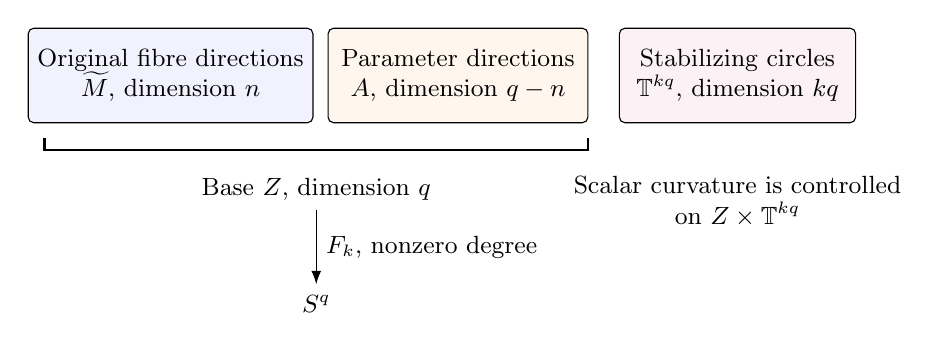
\begin{tikzpicture}[>=Latex,font=\small,
 block/.style={draw,rounded corners=2pt,minimum height=1.2cm,align=center}]
 \node[block,fill=blue!5,minimum width=3.2cm] (m) at (0,0)
   {Original fibre directions\\$\widetilde M$, dimension $n$};
 \node[block,fill=orange!7,minimum width=3.3cm] (a) at (3.65,0)
   {Parameter directions\\$A$, dimension $q-n$};
 \node[block,fill=purple!5,minimum width=3.0cm] (t) at (7.2,0)
   {Stabilizing circles\\$\T^{kq}$, dimension $kq$};
 \draw[thick] (-1.6,-.8)--(-1.6,-.95)--(5.3,-.95)--(5.3,-.8);
 \node[align=center] (z) at (1.85,-1.45)
   {Base $Z$, dimension $q$};
 \draw[->] (z.south)--node[right] {$F_k$, nonzero degree} (1.85,-2.65);
 \node at (1.85,-2.9) {$S^q$};
 \node[align=center] at (7.2,-1.6)
   {Scalar curvature is controlled\\on $Z\times\T^{kq}$};
\end{tikzpicture}
\caption{The local direction splitting after $k$ finite passes. The base
$Z$ is locally a product of original and parameter directions; no global
product decomposition is asserted. The inverse-metric trace uses only the
$n$ original directions. The sphere map uses the full base of dimension
$q$, which is fixed before the number $kq$ of circles is chosen.}
\label{fig:direction-splitting}
\end{figure}


\paragraph{An obstruction independent of the circle count.}
Pulling back a torus tube in $S^q$ gives a compact band $W\subset Z$ carrying
the degree. Doubling $W$ and retaining the circle factors gives a closed
oriented manifold $\operatorname{dbl}(W)\times\T^{kq}$ mapped with nonzero
degree to $S^1\times\T^{q-1}\times\T^{kq}$. The local torical theorem of
Cecchini--Schick requires a
scalar lower bound and a bound on the full differential only on the full
preimage of one connected open target arc. The doubled metric therefore needs
to agree with the constructed metric only there. Constant enlargement of the
stabilizing circles controls their joint projection without scalar loss.
\Cref{sec:obstruction} derives
an obstruction threshold depending on $q$ and $\kappa$, but not on the
number $kq$ of circles. We first choose $R$ large enough to control the total
fibre scalar loss, thereby fixing $q$ and all comparison data, and then choose a
sufficiently large finite $k$ to contradict this obstruction.

\subsection{Consequences}

For a connected aspherical manifold, the classifying map is a homotopy
equivalence. Thus every closed connected oriented aspherical manifold is
rationally essential. The main theorem gives the following consequence, with the
nonorientable case obtained from the orientation double cover.

\begin{corollary}[The Gromov--Lawson aspherical conjecture]
\label{cor:aspherical}
No closed smooth aspherical manifold, whether orientable or not, admits a
Riemannian metric of strictly positive scalar curvature.
\end{corollary}

For nonnegative scalar curvature, the corresponding statement determines
the given metric.

\begin{corollary}[Aspherical nonnegative-scalar-curvature rigidity]
\label{cor:aspherical-flat}
Let $g$ be a Riemannian metric of nonnegative scalar curvature on a closed
smooth aspherical manifold $M$, not necessarily oriented. Then $g$ is flat.
\end{corollary}

Both aspherical statements apply componentwise and have no spin assumption.
In dimensions zero and one scalar curvature vanishes
identically, and every metric is flat. Gromov already noted the rigidity
implication conditionally on the aspherical positive-scalar-curvature
obstruction \cite[Section~3, following Conjecture~B]{GromovDozen2018}.
Here the proof combines \cref{lem:scalar-reduction} with the compact-manifold
consequence of the Cheeger--Gromoll splitting theorem.

A nonzero-degree map to an aspherical target forces rational essentiality by
naturality of classifying maps; no injectivity or surjectivity condition on
the induced map of fundamental groups is needed. The following is the
oriented form of the target-map conjecture recorded by Chodosh and Li
\cite[Conjecture~18]{ChodoshLiSurvey2023}. Their survey also states the
connected-sum obstruction in dimensions four and five as a consequence of
Gromov's work \cite[Theorem~17]{ChodoshLiSurvey2023}.

\begin{corollary}[Oriented target-map obstruction]
\label{cor:degree-aspherical}
Let $M^n$ and $N^n$ be closed connected oriented smooth manifolds of
dimension $n\ge2$, with $N$ aspherical. If a continuous map $f:M\to N$
has nonzero ordinary oriented degree $d\in\Z\setminus\{0\}$, then $M$
admits no Riemannian metric whose scalar curvature is strictly positive
everywhere.

In particular, if $P^n$ is any closed connected oriented smooth manifold,
the oriented connected sum $N\#P$ admits no such metric.
\end{corollary}

For a closed connected oriented $n$-manifold, its \emph{real simplicial
volume} is
\[
 \|M\|=\inf\left\{\sum_i|a_i|:
       \sum_i a_i\sigma_i\text{ is a real singular cycle representing }[M]\right\}.
\]
Positive simplicial volume implies rational essentiality, by the
bounded-cohomology mapping theorem and duality for this seminorm
(\cref{lem:essentiality}). Therefore rational inessentiality implies zero
simplicial volume. The converse fails: a positive-dimensional torus is
rationally essential but has zero simplicial volume, as follows from its
self-covers of degree greater than one. Its flat metric also shows why
strict positivity in \cref{thm:main} cannot be replaced by nonnegative
scalar curvature. For simplicial volume the nonnegative hypothesis does
suffice.

\begin{corollary}[Simplicial-volume vanishing]
\label{cor:simplicial}
Every closed oriented smooth manifold of positive dimension
admitting a Riemannian metric of nonnegative scalar curvature has zero
real simplicial volume.
\end{corollary}

On each connected component, \cref{sec:reductions} reduces a
nonnegative-scalar-curvature metric to either a positive-scalar-curvature
metric or a Ricci-flat metric. The positive branch uses \cref{thm:main};
the Ricci-flat branch uses volume comparison and amenability, without
requiring rational inessentiality in that case.

\subsection{The obstruction problem and earlier work}

Two approaches have shaped scalar-curvature obstructions. Schoen and Yau
used stable two-sided minimal hypersurfaces and conformal deformation to
transfer positive scalar curvature to lower dimensions
\cite{SchoenYauStructure1979,SchoenYauIncompressible1979}. Their original
obstructions requiring no spin assumption apply in dimensions at most seven,
including to manifolds mapping with nonzero degree to tori. Gromov and Lawson
developed Dirac-operator obstructions using enlargeability and relative
indices on complete manifolds \cite{GromovLawson1983}. Their 1983
enlargeability convention requires oriented spin coverings, and their compact
obstruction has no upper dimension bound. The later geometric convention
used above omits this spin requirement. The spin condition in geometric
index applications and the regularity of minimizing hypersurfaces are thus
different constraints.

More recently, Chodosh and Li established the aspherical obstruction in
dimensions four and five using generalized soap bubbles
\cite{ChodoshLi2024}. Gromov independently treated the closed
five-dimensional case, and also complete-manifold domination problems under
properness and uniform-positivity or decay hypotheses
\cite{GromovAsphericalFive2020}.
\Cref{cor:aspherical} establishes the closed-aspherical statement in every
dimension.

The homological formulation in \cref{thm:main} concerns more manifolds than
the aspherical class. Hanke explicitly formulates the conjecture that
rationally essential manifolds do not admit positive scalar curvature
\cite[Definition~2.8 and Conjecture~2.9]{Hanke2011}. It is also the
classifying-map form, for closed oriented sources, of Gromov's conjecture
that a nontorsion homology class in the classifying space of a countable group
cannot be the image of the fundamental class of a positive-scalar-curvature manifold
\cite[Section~1.5, \(\lbrack\mathrm{Sc}\not>0\rbrack\), p.~19]{Gromov2023}.
The numbered sections cited from that work refer throughout to the author's
arXiv version~6. Yau also posed this homological obstruction in his survey
\cite[p.~265]{Yau2000}.

Gromov introduced simplicial volume and its bounded-cohomology description
in \cite{Gromov1982}. His quantitative scalar-curvature/simplicial-volume
conjecture asks for a dimension-dependent upper bound on simplicial volume in
terms of Riemannian volume under a fixed scalar-curvature lower bound
\cite[Section~3.13]{Gromov2023}. Rescaling a nonnegative-scalar-curvature
metric in such a comparison would force zero simplicial volume.
\Cref{cor:simplicial} proves this qualitative vanishing consequence.
The quantitative comparison remains a separate question.

Recent work of Ma, Wang, Xie, Yu and Zhu proves that nonnegative scalar
curvature forces zero real simplicial volume for closed oriented manifolds
with spin universal cover \cite[Corollary~1.2]{MaWangXieYuZhu2026}. Their
stated version has no further group-decay assumption. This conclusion
controls the simplicial norm, rather than the rational classifying image.
Bi and Zhu develop singular hypersurface descent and rule out positive scalar
curvature on closed oriented enlargeable and overtorical manifolds, where an
$n$-manifold is overtorical if it admits a nonzero-degree map to $\T^n$
\cite[Theorems~A and~B]{BiZhu2026}. Their theorem for complete oriented
sources and complete oriented enlargeable targets retains properness,
nonzero-degree and Lipschitz hypotheses and rules out a uniform positive
scalar lower bound.
Under strict positive scalar curvature,
\cref{thm:main} gives rational classifying-image vanishing without these
geometric-largeness or spin-cover hypotheses.

The terminal geometric input here is the local torical theorem of Cecchini
and Schick \cite[Theorem~1.14(1)]{CecchiniSchick2021}. It has no spin assumption
or upper dimension bound, and requires both the scalar lower bound and the
full differential bound only on the full preimage of one connected open target
arc. Its higher-dimensional proof uses the minimal-slicing theory of Schoen
and Yau \cite{SchoenYau2017}.

\Cref{sec:reductions} records the degree conventions and the nonnegative
scalar-curvature reduction. \Cref{sec:comparison} constructs the comparison
data, and \cref{sec:graph-calculus,sec:graph-existence,sec:shortening}
establish the graph stabilization and shortening estimates.
\Cref{sec:obstruction} supplies the stabilized obstruction.
Finally, \cref{sec:main-proof} combines these results and proves the four
corollaries.

\section{Conventions and the nonnegative scalar-curvature reduction}
\label{sec:reductions}

We record the degree conventions for the comparison construction and reduce
nonnegative scalar curvature to the positive and Ricci-flat cases used in the
corollaries. All manifolds and metrics are smooth. A closed manifold is compact
and has no boundary. Unless stated otherwise, manifolds are oriented.
Fundamental classes are taken with the indicated coefficients; we use the same
symbol $[M]$ for
an integral fundamental class and its images under extension of coefficients.
The Laplacian is $\Delta=\diver\nabla$, and a round sphere has positive scalar
curvature. For a hypersurface with unit normal $\nu$, our second fundamental
form is $\mathrm{II}(X,Y)=\langle\nabla_X\nu,Y\rangle$ and its mean curvature
is its trace. These conventions fix the signs in the graph calculations below.
We give $S^d$ its unit round metric and write
$\T^b=(\R/2\pi\Z)^b$ for the standard flat torus.

\subsection{Fundamental classes and degree}

Throughout the proof, $\Gamma=\pi_1(M)$ and $c_M:M\to B\Gamma$
have the meaning fixed in \cref{sec:introduction}. No finite-dimensional
model for $B\Gamma$ is assumed. Disconnected closed manifolds are treated
one component at a time; compactness leaves only finitely many components.

For a possibly noncompact oriented $d$-manifold $Y$, a smooth map
$F:Y\to S^d$ that is equal to one value $*\in S^d$ outside a compact set has
a well-defined degree. One may compute it as the signed number of preimages
of any regular value different from $*$. Those preimages are contained in a
compact set. Equivalently, pull back a compactly supported top-degree class on
$S^d\setminus\{*\}$ and evaluate it on the locally finite fundamental class
of $Y$. This definition also permits disconnected $Y$: only finitely many
components can meet the compact region on which $F$ is nonconstant. We use
\emph{constant outside a compact set} in this sense, rather than assigning a
linear meaning to compact support for a sphere-valued map.

We also use the ordinary oriented local degree $\deg(G,\Omega,0)$ for a
smooth map from an oriented $q$-manifold to $\R^q$, where $\Omega$ is a
precompact open set and $0\notin G(\partial\Omega)$. Smoothness of
$\partial\Omega$ is unnecessary. A homotopy whose boundary values avoid zero
preserves this degree. More generally, if they avoid a fixed ball, composition
with a degree-one map $\R^q\to S^q$ constant outside that ball gives a
sphere-valued map of the same degree, extending constantly across the boundary
of $\Omega$.

\begin{lemma}[Simplicial volume detects rational essentiality]
\label{lem:essentiality}
If a closed connected oriented manifold $M^n$ has positive real simplicial
volume, then $(c_M)_*[M]\ne0$ in $H_n(B\Gamma;\Q)$.
\end{lemma}

\begin{proof}
The bounded-cohomology mapping theorem identifies real bounded cohomology of
$M$ with that of $B\Gamma$ by pullback along $c_M$. The duality between
bounded cohomology and the $\ell^1$-seminorm implies that
$\|M\|>0$ supplies a bounded class whose ordinary cohomology image evaluates
nontrivially on $[M]$. These are the mapping and duality results of
\cite{Gromov1982}; neither requires a spin structure.

If $(c_M)_*[M]$ vanished rationally, its real image would vanish. Every bounded
class pulled back from $B\Gamma$ would then evaluate trivially on $[M]$, a
contradiction. In dimension one, real bounded cohomology already vanishes and
the assertion is vacuous; the direct circle argument below also suffices.
\end{proof}

\subsection{The scalar-flat alternative}

\begin{lemma}[Positive scalar curvature or Ricci flatness]
\label{lem:scalar-reduction}
Let $M$ be closed and connected, not necessarily oriented, and suppose that
$g$ has nonnegative scalar curvature. Either $M$ admits a metric of strictly positive scalar curvature,
or $g$ is Ricci-flat. In the Ricci-flat case, if $M$ is oriented and has
positive dimension, then $\|M\|=0$.
\end{lemma}

\begin{proof}
Run the short-time Ricci flow starting at $g$. Short-time existence on closed
manifolds and the scalar evolution equation give
\begin{equation}\label{eq:scalar-evolution}
 \partial_t\Scal=\Delta\Scal+2|\Ric|^2.
\end{equation}
See \cite[Theorem~5.2.1 and Proposition~2.5.4]{Topping2006} for these
statements in arbitrary dimension, and \cite{Hamilton1982} for the
Ricci-flow framework. The maximum principle
preserves nonnegativity. If the initial scalar curvature is positive at one
point, the strong maximum principle makes it positive everywhere at any
sufficiently small later time. If it is initially identically zero but the
Ricci tensor is nonzero at a point, \eqref{eq:scalar-evolution} gives a
strictly positive initial time derivative there. At a sufficiently small positive time $t_1$, scalar curvature is
therefore positive at that point. Applying the strong maximum principle
from $t_1$ produces a metric of positive scalar curvature everywhere at
a later time. Thus failure of this alternative
forces $\Ric_g=0$.

For the final assertion, suppose that $g$ is Ricci-flat, that $M$ is
oriented, and that $n=\dim M>0$. We use the orbit-packing argument
of Milnor \cite[Theorem~1]{Milnor1968}. Its complete universal Riemannian cover
$(\widetilde M,\widetilde g)$ has nonnegative Ricci curvature. Fix
$x\in\widetilde M$ and a finite generating set of $\Gamma$. There is a
constant $D$ such that
\[
 d(x,\gamma x)\le D|\gamma|
 \qquad(\gamma\in\Gamma),
\]
where $|\gamma|$ is word length. Choose a positive radius $r$ for which the
balls $B(\gamma x,r)$, $\gamma\in\Gamma$, are disjoint. To choose $r$, take a sufficiently small metric ball about the image of
$x$ contained in an evenly covered neighborhood. The radius-$r$ balls
about its lifts lie in distinct sheets and are therefore disjoint. All these
balls have the same positive volume, say $v_r$. The orbit balls with
$|\gamma|\le k$ lie in $B(x,Dk+r)$. Bishop--Gromov comparison \cite[Theorem~4.1]{Wei2007} therefore gives
\[
 \#\{\gamma:|\gamma|\le k\}\,v_r
 \le \Vol B(x,Dk+r)\le \omega_n(Dk+r)^n.
\]
Thus $\Gamma$ has polynomial word growth. Write
$b(k)=\#B_\Gamma(1,k)$. There are integers $k_j\to\infty$ such that
$b(k_j+1)/b(k_j)\to1$. Otherwise, some $\varepsilon>0$ would satisfy
$b(k+1)/b(k)\ge1+\varepsilon$ for all sufficiently large $k$, forcing
exponential growth. For each generator $s$,
\[
 \#\bigl(sB_\Gamma(1,k_j)\mathbin\triangle B_\Gamma(1,k_j)\bigr)
 \le2\bigl(b(k_j+1)-b(k_j)\bigr).
\]
These balls form a F\o lner sequence, so $\Gamma$ is amenable. This
uses only the growth bound, without a structural classification of groups
of polynomial growth. Real bounded
cohomology of an amenable group vanishes in positive degrees
\cite[Sections~3.0--3.1]{Gromov1982}. The mapping
theorem and duality used in \cref{lem:essentiality} now imply
$\|M\|=0$.
\end{proof}

Every closed connected oriented one-manifold is a circle. Its self-cover of
degree two and functoriality of the simplicial seminorm give
$2\|S^1\|\le\|S^1\|$, hence $\|S^1\|=0$. Consequently, to prove the
simplicial-volume theorem in every positive dimension, it remains to show
that a positive-scalar-curvature manifold of dimension at least two is
rationally inessential. Compactness lets us write its scalar lower bound as
$\Scal_M\ge\kappa>0$.

\section{Compact pairings and comparison coordinates}
\label{sec:comparison}

The construction in this section is topological.  A Riemannian metric is
used only to measure derivatives in the direction of the original
manifold.  In particular, no curvature hypothesis enters the following
statement. For a vector, $\norm{\cdot}_\infty$ is the maximum of the
absolute coordinate values. Bounds asserted on a set are pointwise;
uniform norms take the supremum over the domain.

\begin{theorem}[Comparison data from rational essentiality]
\label{thm:comparison-data}
Let $(M^n,g_M)$ be a closed connected oriented Riemannian manifold,
$n\ge2$, let $\Gamma=\pi_1(M)$, and suppose that its classifying map
$c_M:M\to B\Gamma$ satisfies
\[
 (c_M)_*[M]\ne0\quad\text{in }H_n(B\Gamma;\Q).
\]
There are constants $J>0$ and $R_0\ge1$ such that, for every real
$R\ge R_0$, there exist a closed oriented smooth manifold $A$, a
principal left $\Gamma$-cover $\widehat A\to A$, and an integer
$q=n+\dim A>n$ with the following properties.  The diagonal cover
\[
 Z=(\widetilde M\times\widehat A)/\Gamma\longrightarrow M\times A
\]
is oriented and has dimension $q$.  There are a smooth compactly
supported map $G:Z\to\R^q$ and a relatively compact open set
$\Omega\subset Z$ such that
\begin{equation}
\label{eq:comparison-degree}
 \deg(G,\Omega,0)\ne0,
 \qquad \norm{G}_\infty>3\quad\text{on }\partial\Omega,
\end{equation}
and
\begin{equation}
\label{eq:comparison-bounds}
 \max_{1\le i\le q}\sup_Z\abs{d_{\widetilde M}G_i}_{g_M}
 \le\frac JR,
 \qquad \log q\le JR.
\end{equation}
Write $\pi_Z:Z\to M\times A$ for the covering projection. Its
differential gives a global splitting
\[
 TZ=E_M\oplus E_A,\qquad
 E_M=(d\pi_Z)^{-1}(TM\oplus0),\qquad
 E_A=(d\pi_Z)^{-1}(0\oplus TA).
\]
The bundle $E_M$ is tangent to the $\widetilde M$ fibres of $Z\to A$,
and $E_A$ is the flat lift of the parameter directions. We write
$d_{\widetilde M}G_i=dG_i|_{E_M}$. For each fixed $R$, after choosing any
smooth metric on $A$, all derivatives of $G$ in the lifted product
geometry are bounded.  No bound uniform in $R$ is asserted for
parameter derivatives or for derivatives of order greater than one.
The covers and the parameter manifolds need not be connected.
\end{theorem}

We use rational coefficients for the chain constructions in this
section. A principal left $\Gamma$-cover is a covering on which $\Gamma$
acts freely by deck transformations and transitively on each fibre. Every
diagonal quotient below uses left actions in both factors.  Orientations
on covers are lifted from the base, so all deck transformations preserve
them.

The construction proceeds as follows. An auxiliary closed manifold $C$
provides a finite parameter space for a compactly supported group-cohomology
pairing. Distance profiles then supply $q$ scalar coordinates, with $q$
initially only a row count. Relative duality produces a complementary
rational class of degree $q-n$. Oriented realization of a nonzero multiple,
followed by doubling, gives the parameter manifold $A$. Thus the final cover has
exactly the dimension needed for a local degree, $n+\dim A=q$; the topology
of the realized $A$ does not alter the previously chosen row count.

\subsection{Probability maps and a finite parameter manifold}

Fix a finite symmetric generating set of $\Gamma$, and write
$d_\Gamma$ for its left-invariant word metric.  For $a\ge0$, let
$\mathcal K_a$ be the Rips complex realized as finite probability vectors
$t=(t_\gamma)_{\gamma\in\Gamma}$ whose nonempty support has diameter at
most $a$.  This complex is locally finite, finite dimensional, and
cocompact under left translation.  The action is proper, although it
need not be free when $\Gamma$ has torsion.

\begin{lemma}[A proper probability map]
\label{lem:probability-map}
There are $s\ge1$, $H<\infty$, a smooth equivariant probability map
$h:\widetilde M\to\mathcal K_s$, and an equivariant simplicial map
$h_0:\widetilde M\to\mathcal K_s$ such that
\begin{enumerate}
\item the coordinate functions of $h$ are smooth and locally supported
on finitely many labels, and $\abs{dh}_{\ell^1}\le H$;
\item $h$ and $h_0$ are joined by an equivariant homotopy that is proper
as a map $\widetilde M\times[0,1]\to\mathcal K_s$;
\item there is an invariant alternating homogeneous rational group
$n$-cocycle $\omega$ whose evaluation on the labelled fundamental
simplices of $M$ is nonzero.
\end{enumerate}
\end{lemma}

\begin{proof}
Choose a finite smooth triangulation of $M$ by the Cairns--Whitehead
theorem \cite{Cairns1934,Whitehead1940}; see also
\cite[Theorem~10.6]{Munkres1966}. Label the vertex lifts
equivariantly by elements of $\Gamma$, making one arbitrary choice for
each vertex downstairs.  Barycentric coordinates define the labelled
simplicial map $h_0$.  A smooth partition of unity subordinate to the
open vertex stars, lifted equivariantly, gives $h$; weights with the same
label are added.  At each point the labels that occur belong to the
vertices of one lifted simplex.  Cocompactness bounds their word
diameters by a fixed $s$, and it also bounds the $\ell^1$-operator norm
of $dh$ by a fixed $H$.  Linear interpolation of the weights stays in
$\mathcal K_s$.

For completeness, this entire homotopy is proper.  If $Q\subset
\widetilde M$ is compact with $\Gamma Q=\widetilde M$, its image during
the homotopy is compact.  Given a compact $B\subset\mathcal K_s$,
properness of the $\Gamma$-action allows only finitely many translates
of that image to meet $B$.  The inverse image of $B$ is therefore a
closed subset of finitely many translates of $Q\times[0,1]$.

Choose a class in $H^n(B\Gamma;\Q)$ pairing nontrivially with
$(c_M)_*[M]$, and represent it on the homogeneous bar resolution.  On
tuple chains, signed permutation averaging is an equivariant chain map
lifting the identity of the augmentation.  It is equivariantly chain
homotopic to the identity on this free resolution.  Antisymmetrizing
the representative thus gives a cocycle $\omega$ in the same class.
It vanishes on repeated labels and restricts to a simplicial cocycle on
every $\mathcal K_a$.

Give the vertices of $M$ a global order.  Sending an ordered lifted
simplex to its tuple of labels gives an augmentation-preserving
equivariant chain map into the bar resolution.  Such a map is unique
up to equivariant chain homotopy: inductively, the difference in each
degree is a cycle in the exact target resolution, and freeness of the
source chains permits equivariant fillings.  Comparison with the chain
map induced by a classifying map shows that evaluation of $\omega$ on
these labelled fundamental simplices is precisely its pairing with
$(c_M)_*[M]$, and hence is nonzero.
\end{proof}

The detecting cocycle is now fixed. To construct a finite smooth parameter
space carrying its compact pairing, we need a free auxiliary group action.
The ordinary Rips action may have torsion stabilizers; keeping the order
of every simplex removes them without requiring contractibility.

Fix henceforth $R\ge s+1$ and set
\begin{equation}
\label{eq:comparison-scales}
 L=100R.
\end{equation}
All auxiliary spaces constructed at this scale may depend on $L$.
Let $\mathcal O_L$ be the semisimplicial complex with one simplex for
each ordered tuple of distinct group elements of diameter at most $L$;
faces are obtained by deleting slots, and different orderings are not
identified.  Projection of a tuple to its probability simplex gives
$\pi:\mathcal O_L\to\mathcal K_L$.  On chains it has the equivariant
section
\begin{equation}
\label{eq:ordered-section}
 \sigma[v_0,\ldots,v_j]
 =\frac1{(j+1)!}\sum_{\varpi\in S_{j+1}}
    \sgn(\varpi)(v_{\varpi(0)},\ldots,v_{\varpi(j)}).
\end{equation}
Counting the positions of a deleted entry verifies that $\sigma$ is a
chain map, and $\pi_\#\sigma=\id$.

\begin{lemma}[A parameter thickening]
\label{lem:parameter-thickening}
Put $v_0=\dim\mathcal O_L$.  There are a closed oriented smooth
$d$-manifold $C$, with $d\le2v_0+2$, a principal left $\Gamma$-cover
$\widehat C\to C$, and equivariant maps
\[
 \mathcal O_L\xrightarrow{i}\widehat C
 \xrightarrow{r}\mathcal K_L,
 \qquad r i=\pi.
\]
Moreover $v_0\le\abs{B_\Gamma(1,L)}$.
\end{lemma}

\begin{proof}
A point in the realization of $\mathcal O_L$ belongs to the interior of
a unique minimal-dimensional ordered simplex.  A group element fixing
the point must preserve that ordered simplex, hence must fix its labels
slot by slot.  It is therefore the identity.  This also proves freeness
at points represented on faces; face identifications do not identify
distinct orderings of the minimal simplex.  Local finiteness and the
word-metric bound make the action proper and its quotient finite.
Thus $\mathcal O_L\to\mathcal O_L/\Gamma$ is a principal cover, including
when $\Gamma$ has torsion.  The quotient has a finite polyhedral
subdivision.  A simplex has at most $\abs{B_\Gamma(1,L)}$ vertices after
one of its vertices is translated to the identity, proving the
dimension bound.

Embed the finite polyhedron $\mathcal O_L/\Gamma$ in
$\R^{2v_0+1}$ and choose an open neighborhood retracting onto it.
Choose a compact smooth domain inside that neighborhood containing the
polyhedron in its interior, and double the domain.  Folding the double
to the domain followed by the neighborhood retraction gives a
retraction from a closed oriented manifold $C$ onto
$\mathcal O_L/\Gamma$.  Its dimension satisfies the stated bound.
Pull back the principal cover along this retraction.  The inclusion
of the polyhedron lifts to $i$, while the pullback projection followed
by $\pi$ gives $r$.  Their composition has the required value.
\end{proof}

Fix a smooth metric on $C$ and lift it to $\widehat C$.  A useful
consequence of continuity and cocompactness is the following uniform
common-label property: sufficiently small subsets of $\widehat C$ have
images under $r$ with a label common to every positive support.  Indeed,
at any point a positive coordinate remains positive on a neighborhood;
a finite cover downstairs gives a uniform neighborhood size upstairs.

\begin{lemma}[A controlled map to dual chains]
\label{lem:dual-carrier}
One can triangulate $C$ so finely that the lifted triangulation has
the following properties:
\begin{enumerate}
\item the union of the supports of $r(o)$ over any closed primal
simplex has diameter at most $2L$;
\item there is an augmentation-preserving equivariant chain map
\[
 \mathcal F:C_*(\mathcal O_L)\longrightarrow
 C_*^{\mathrm{dual}}(\widehat C)
\]
with finite output, such that if a dual cell to a primal simplex
$\tau$ occurs in $\mathcal F(e)$, then every label of every $r(o)$,
$o\in\tau$, is within $2L$ of every vertex of $e$.
\end{enumerate}
\end{lemma}

\begin{proof}
Use a sufficiently fine smooth triangulation, so that both primal
simplices and closed dual blocks have arbitrarily small mesh.  If all
images over a primal simplex share a label, every pair of labels in
their union is within $2L$.  This gives the first assertion.

We describe the chain construction explicitly.  The regular dual-cell
decomposition has closed cells that are balls and cellular subcomplexes.
Subdivide it barycentrically.  A simplex $s'$ of this subdivision is a
flag of dual cells; let $B(s')$ be the closure of its largest cell.
This is the unique minimal closed dual cell containing $s'$.  For a
face $t'$ of $s'$ we have $B(t')\subset B(s')$, so these closed balls
form a face-compatible acyclic carrier.

There is an augmentation-preserving chain map from the subdivision
chains to dual-cell chains carried by $B$.  To construct it, send a
vertex to a dual zero-cell in its carrier with coefficient one.  If
the map has been defined below dimension $j$, the image of the boundary
of a $j$-simplex is an augmented cellular cycle in its carrier, because
all face carriers are contained there.  Fill the cycle within this
contractible cellular subcomplex.  Make all choices on simplex orbits
and translate.  The deck action on the subdivision is free, so this is
equivariant.  Each carrier is finite, and hence each output is finite.

Now subdivide $\mathcal O_L$ equivariantly and approximate the actual
map $i$ closely by a simplicial map into the subdivision of the dual
decomposition. Choose the target stars inside sufficiently small evenly
covered balls. Simplicial approximation on the finite quotients can then
be joined to the original map by a homotopy staying in those stars.
Lifting that homotopy from $i$ gives an equivariant simplicial endpoint
that remains uniformly close to $i$ upstairs. Equivalently, one may choose
the stars directly on free vertex orbits. Compose source subdivision,
this simplicial chain map, and the carrier map just constructed.  This
defines $\mathcal F$.  Contractibility of $\mathcal O_L$ is not needed:
the only fillings take place inside the target carrier balls.

Consider a dual cell occurring on an original simplex $e$.  Its
carrier lies within a small mesh error of $i(z)$ for some $z\in e$.
The primal simplex $\tau$ dual to that cell meets it at its barycenter;
small primal mesh therefore puts every $o\in\tau$ within another small
error of such an $i(z)$.  Choose all meshes and the approximation close
enough to apply the common-label property to the pair $o,i(z)$.  A
common label $v$ belongs both to $r(o)$ and to $r(i(z))$.  Since
$ri=\pi$, the latter support consists of vertices of $e$.  For a label
$\gamma$ of $r(o)$ and a vertex $w$ of $e$, we obtain
\[
 d_\Gamma(\gamma,w)
 \le d_\Gamma(\gamma,v)+d_\Gamma(v,w)\le L+L.
\]
This proves the second assertion.
\end{proof}

\subsection{A compactly supported pairing}

For $0\le a\le L$ define
\[
 D_a=(\mathcal K_a\times\widehat C)/\Gamma,
 \qquad
 X=(\widetilde M\times\widehat C)/\Gamma.
\]
Both spaces project to $C$.  The oriented manifold $X$ has dimension
$n+d$, and the probability map induces the graph map
\[
 \begin{array}{ccc}
 X&\xrightarrow{\Phi_h}&D_L\\
 \downarrow&&\downarrow\\
 C&=&C
 \end{array}
 \qquad
 \Phi_h([\widetilde x,o])=[h(\widetilde x),o].
\]
This map is proper, as is the graph homotopy induced by the homotopy in
\cref{lem:probability-map}.  To see joint properness, cover compact $C$
by finitely many compact subsets contained in trivializing charts of
$\widehat C$.  In each chart a compact subset of $D_L$ has compact
first-factor projection.  Joint properness of the probability homotopy
controls the preimage in the $\widetilde M$ factor, and the parameter subset is compact.
A finite union gives the assertion.

The chain construction has a specific target: cap each simplex with the
detecting cocycle, retain the correct augmentation in degree $n$, and keep
the complementary dual cells close to the original labels. The following
lemma packages these properties before cellular duality is applied.

\begin{lemma}[A controlled cap operation]
\label{lem:controlled-cap}
There are equivariant linear maps with finite output
\begin{equation}
\label{eq:cap-chain-map}
 \begin{gathered}
 T_j:C_j(\mathcal K_L;\Q)\longrightarrow
 C_{j-n}^{\mathrm{dual}}(\widehat C;\Q),\qquad j\ge0,\\
 \partial T_j=(-1)^nT_{j-1}\partial,\qquad j\ge1,
 \end{gathered}
\end{equation}
where chain groups in negative degrees are zero. For every oriented
$n$-simplex $e$, the augmentation of $T_n(e)$ is $\omega(e)$. For every
oriented $j$-simplex $e$, if a dual cell to a primal simplex $\tau$ occurs
in $T_j(e)$, then every label of
$r(o)$, for every $o\in\tau$, is within $3L$ of every vertex of $e$.
\end{lemma}

\begin{proof}
On an oriented $j$-simplex $e=[v_0,\ldots,v_j]$ define the averaged
Alexander--Whitney diagonal by
\[
 \Delta_{\mathrm{AW}}e
 =\frac1{(j+1)!}\sum_{\varpi\in S_{j+1}}\sgn(\varpi)
   \sum_{k=0}^j
 [v_{\varpi(0)},\ldots,v_{\varpi(k)}]
 \otimes[v_{\varpi(k)},\ldots,v_{\varpi(j)}].
\]
Each ordering gives the usual diagonal on that simplex and its faces.
Restriction of a uniformly chosen ordering to a face is again uniformly
distributed, so the average commutes with the boundary. It is equivariant,
and both factors in every term are faces of $e$.

Apply $\omega$ to the first factor of degree $n$ and $\mathcal F\sigma$
to the second factor, and call the resulting graded map $T$. Its outputs
are finite. In the tensor boundary, the sum of terms from the first factor
vanishes after evaluation by $\omega$ because $\delta\omega=0$. The boundary in the
second factor carries the sign $(-1)^n$, proving
\eqref{eq:cap-chain-map}. When $j=n$, each contributing second factor is a
vertex. Its image under $\mathcal F\sigma$ has augmentation one, while
alternation makes every signed first-factor evaluation equal to $\omega(e)$.
Thus the augmentation of $T_n(e)$ is exactly $\omega(e)$.

Finally, every output of $T_j(e)$ comes from a face of $e$. By
\cref{lem:dual-carrier}, labels over its corresponding primal simplex are
within $2L$ of every vertex of that face. Since $e$ has diameter at most
$L$, they are within $3L$ of every vertex of $e$.
\end{proof}

Cellular duality will turn the finite output of $T$ in dual chains into primal
cochains. Its support bound will make the resulting product class compactly supported,
and its augmentation will recover the original cocycle pairing.

\begin{proposition}[Compact diagonal pairing]
\label{prop:compact-pairing}
There are a compact set $K_*\subset D_L$ and a class
\[
 u\in H^{n+d}(D_L,D_L\setminus K_*;\Q)
\]
such that
\begin{enumerate}
\item if $[t,o]\in K_*$, every label of $t$ is within $7L$ of
every label of $r(o)$;
\item the compactly supported evaluation
\begin{equation}
\label{eq:compact-pairing-nonzero}
 \ip{\Phi_h^*u,[X]_{\mathrm{lf}}}\ne0
\end{equation}
is nonzero.
\end{enumerate}
Here $[X]_{\mathrm{lf}}$ is the locally finite fundamental class.
\end{proposition}

\begin{proof}
Cellular duality on the oriented cover identifies finite dual chains
of degree $k$ with compactly supported primal cochains of degree
$d-k$.  Write this identification as $I$, choosing the degree signs
so that $\delta I=I\partial$.  At degree zero choose the sign for which
evaluation on the oriented locally finite fundamental cycle is the
augmentation; the remaining degree signs are then determined
successively by the boundary--coboundary identity.  On product cells,
define a cochain $U$ of degree $n+d$ by
\begin{equation}
\label{eq:product-cocycle}
 \begin{split}
 U(e^j,e'^{\,n+d-j})&=a_j I(T(e))(e'),\\
 a_n&=1,\qquad
 a_j=(-1)^{j+n+1}a_{j-1}\quad(j>n),
 \end{split}
\end{equation}
and set it to zero outside the indicated chain degrees.  The cochain
is invariant under simultaneous translation and thus descends to
$D_L$.  The product-cell structure is valid even if the action on
$\mathcal K_L$ has inversions: the freely lifted second-factor cells
give trivial stabilizers of product cells.

On a product cell of bidegree $(j,n+d+1-j)$, the two terms in
$\delta U$ are $a_{j-1}IT(\partial e)$ and
$(-1)^ja_jI\partial T(e)$.  By \cref{eq:cap-chain-map}, their
coefficients relative to $IT(\partial e)$ are
$a_{j-1}$ and $(-1)^{j+n}a_j$, which cancel.  Thus $U$ is a cocycle.

Call a product cell \emph{far} if all distances between vertices of
its first simplex and labels of $r$ over its closed second simplex
are greater than $4L$.  This condition is inherited by faces and is
translation invariant, so the far cells form a subcomplex
$D_{\mathrm{far}}\subset D_L$. The support bound in
\cref{lem:controlled-cap} shows that
$U$ vanishes on it.  Let $K_*$ be the union of the closures of all
non-far cells in the quotient.  There are only finitely many such
cells: after fixing a second-factor simplex from finitely many orbit
representatives, non-farness puts some first-factor vertex within
$4L$ of a label in a fixed finite set; the other vertices lie within
$L$ of that vertex.  Local finiteness of the word metric gives only
finitely many choices.

The same argument gives the required support bound.  One pair of
labels in a non-far product is within $4L$, the first simplex has
diameter at most $L$, and the union of second-factor labels has
diameter at most $2L$.  Every pair in its closure is consequently
within $4L+L+2L=7L$.  Furthermore
$D_L\setminus K_*\subset D_{\mathrm{far}}$, so the relative cellular
class of $U$ induces the required class $u$.

It remains to compute the pairing.  By proper homotopy invariance of
compactly supported cohomology, replace $h$ by $h_0$ and write
$\Phi_0$ for the resulting graph map.  On the product cell structure
of $X$, each open cell maps to an open product cell, possibly of
smaller dimension.  Thus
$X_{\mathrm{far}}=\Phi_0^{-1}(D_{\mathrm{far}})$ is a subcomplex.
Every cell not in it lies in the compact set $\Phi_0^{-1}(K_*)$, and
there are finitely many such cells by local finiteness.  The locally
finite fundamental class maps successively to
\[
 H_{n+d}(X,X\setminus\Phi_0^{-1}(K_*);\Q)
 \longrightarrow H_{n+d}(X,X_{\mathrm{far}};\Q).
\]
In the latter group it is represented by the finite product
fundamental cellular chain modulo $X_{\mathrm{far}}$.  Its coefficient
on each remaining top cell is the local orientation coefficient,
as follows by restricting further to local homology at an interior
point.  Hence evaluation by the relative cellular cocycle computes
the desired compact pairing.

Only bidegree $(n,d)$ contributes.  For each oriented fundamental
top simplex of $M$, choose one lift and sum over all oriented
fundamental top simplices of $\widehat C$.  The latter sum evaluates
$IT(e)$ on the locally finite parameter fundamental cycle and equals
the augmentation of $T(e)$, namely $\omega(e)$.  Collapsed labelled
top simplices contribute zero.  The total is exactly the nonzero
evaluation from \cref{lem:probability-map}, proving
\cref{eq:compact-pairing-nonzero}.
\end{proof}

\subsection{Distance profiles}

The compact pairing detects the original fundamental class. We next encode
its supporting region by finitely many scalar coordinates whose fibre
derivatives have a scale-independent bound. Their row count will determine
the dimension of the final parameter manifold only after these estimates
have been fixed.

Choose a finite cover of $C$ by small trivializing charts $U_\lambda$,
with $d+1$ colors and with charts of each color pairwise disjoint.
One obtains this by taking open stars of the vertices of a sufficiently
fine barycentric subdivision and coloring them by the dimensions of
the original simplices.  Shrink this finite cover and choose smooth
functions $0\le w_\lambda\le1$, supported in $U_\lambda$, so that at
least one equals one at each point of $C$.  On every sheet over a chart
choose an anchor $g_\lambda(o)\in\Gamma$, constant on the sheet and
equivariant under left translation, which is a common label of $r$
over that sheet.  Thus it is within $L$ of every label of every $r(o)$
there.

For each color and each $b\in B_\Gamma(1,1000L)$ use one row of a
vector $V_o(t)$.  Outside the charts of that color its value is zero;
on the sheet of a chart $U_\lambda$ it is
\begin{equation}
\label{eq:distance-profile-row}
 w_\lambda(\bar o)\sum_{\gamma\in\Gamma}t_\gamma
 \bigl(d_\Gamma(\gamma,g_\lambda(o)b)
             -d_\Gamma(g_\lambda(o),g_\lambda(o)b)\bigr),
 \qquad \bar o=[o].
\end{equation}
The disjointness within each color makes this definition unambiguous.
Compact support of each cutoff inside its chart makes it smooth in
the parameter wherever the probability coordinates are fixed.  Left
invariance of the word metric makes the vector invariant under
simultaneous translation, and hence it is defined on $D_L$.

Pad the vector by zero rows if necessary so that its number $q$ of
coordinates exceeds $n$.  Since the word balls have at most exponential
growth and $d\le2\abs{B_\Gamma(1,L)}+2$, there is a constant $J_1$,
independent of $R$, such that
\begin{equation}
\label{eq:profile-count}
 \log q\le J_1R.
\end{equation}
Choose an even integer $p_R\ge2$ with $q^{1/p_R}\le3$.  The norm
$\norm{\cdot}_{p_R}$ is smooth off zero and satisfies
\begin{equation}
\label{eq:profile-norms}
 \norm{z}_\infty\le\norm{z}_{p_R}\le3\norm{z}_\infty.
\end{equation}

\begin{lemma}[Profile estimates]
\label{lem:distance-profiles}
The map $V:D_L\to\R^q$ has the following properties.
\begin{enumerate}
\item It is continuous and proper, and
$\norm{V}_{p_R}\le24L$ on $K_*$.
\item If $t,t'\in\mathcal K_s$ satisfy
\[
 \max\{\norm{V_o(t)}_\infty,\norm{V_o(t')}_\infty\}\le110L,
 \qquad
 \norm{V_o(t)-V_o(t')}_\infty\le14R,
\]
then the union of their supports has diameter at most $L$.
\item The map
$\mathcal V=V\Phi_h:X\to\R^q$ is smooth.  With $K_0=sH$,
each of its rows satisfies
\[
 \sup_X\abs{d_{\widetilde M}\mathcal V_i}\le K_0,
\]
where $K_0$ is independent of $R$.
\end{enumerate}
\end{lemma}

\begin{proof}
Continuity follows from the coordinate definition and local finiteness.
At any point choose a chart whose cutoff equals one, and use its
$b=1$ row.  This row is the nonnegative average distance to its
anchor $g$.  For $t\in\mathcal K_L$ and any
$\gamma\in\supp t$, the triangle inequality gives
\[
 d_\Gamma(\gamma,g)
 \le\sum_{\gamma'}t_{\gamma'}d_\Gamma(\gamma',g)+L
 \le\norm{V_o(t)}_\infty+L.
\]
Over finitely many trivializing charts, a bound on $V$ therefore
restricts the first-factor labels to finitely many possibilities.
Closed inverse images of compact subsets are consequently compact.
On $K_*$, every input label is within $7L+L=8L$ of the active anchor.
Each distance difference in \cref{eq:distance-profile-row} is bounded
by that distance to the anchor, giving
$\norm{V}_\infty\le8L$, and hence the stated $24L$ bound.

For the second assertion, use a chart of weight one common to both
probabilities and let $g$ be its anchor.  Every label of either
probability is within $110L+s$ of $g$.  In particular a label
$\gamma\in\supp t$ equals $gb$ for one of the rows being used.
In this row the average of $d_\Gamma(\,\cdot\,,\gamma)$ over $t$
is at most $s$.  The row comparison implies that the average over
$t'$ is at most $s+14R$.  Since $\supp t'$ has diameter at most $s$,
every $\gamma'\in\supp t'$ satisfies
\[
 d_\Gamma(\gamma',\gamma)\le14R+2s<L.
\]
This applies to every label of $t$; the within-support distances
already satisfy the bound.

Finally, each row of $\mathcal V$ is locally a finite smooth sum.
In a $\widetilde M$ direction $\sum_\gamma dh_\gamma=0$.  Choose one
label from the current support and subtract its distance profile
before differentiating.  The remaining profile values have
oscillation at most $s$, because the distance function to any fixed
label is $1$-Lipschitz for $d_\Gamma$.  The derivative is thus bounded
by $s\abs{dh}_{\ell^1}\le sH$.  A smooth nonnegative coordinate that
vanishes at the point has zero differential, so zero probability
coordinates introduce no additional labels into this estimate.
\end{proof}

\subsection{From a relative pairing to local degree}

We now have the row count $q$ and its logarithmic bound. Relative duality
will turn the compact pairing into a transverse parameter cycle of
dimension $q-n$. Its intersections with the graph of the coordinate map
will supply the local degree, with different boundary pieces protecting
the two cycles.

Let $E=C\times\R^q$.  The set $V_o(\mathcal K_s)$ depends only on
$\bar o=[o]$, and we define
\[
 \rho(\bar o,y)=\dist_\infty\bigl(y,V_o(\mathcal K_s)\bigr).
\]
This is continuous.  In a trivialization, fixed witnesses give upper
semicontinuity.  For the reverse inequality, a sequence of almost
minimizing witnesses for bounded $y$ has bounded $V$-values; properness
in \cref{lem:distance-profiles} gives a convergent subsequence.  Its
limit is still in the closed subcomplex $\mathcal K_s$, and gives
lower semicontinuity.

Smooth $\rho$ within error $R/10$ on a neighborhood of
$\norm{y}_{p_R}\le110L$, obtaining $\rho_{\mathrm{sm}}$.  By Sard's
theorem \cite{Sard1942}, choose regular transverse levels
\begin{equation}
\label{eq:triad-levels}
 100L<T_0<101L,
 \qquad 5R<d_0<6R,
\end{equation}
also choosing $T_0$ regular for $\norm{\mathcal V}_{p_R}$ on $X$.
The latter function is smooth at these positive levels.  Then
\begin{equation}
\label{eq:compact-triad}
 P=\{(\bar o,y):\norm{y}_{p_R}\le T_0,
                         \ \rho_{\mathrm{sm}}(\bar o,y)\le d_0\}
\end{equation}
is a compact oriented manifold with corners.  Its radial and angular
sides are denoted by $E_R$ and $E_B$, respectively.  They satisfy
\begin{equation}
\label{eq:triad-gaps}
 \rho>4R\ \text{on }E_B,
 \qquad \rho<7R\ \text{throughout }P.
\end{equation}

There is a map $\psi:P\to D_L$ over $C$ with
\begin{equation}
\label{eq:witness-approximation}
 \norm{V\psi(\bar o,y)-y}_\infty<7R.
\end{equation}
Indeed, at each point choose a witness in $\mathcal K_s$ satisfying
this inequality, and continue it as a constant probability vector in
a small sheet trivialization.  It remains a witness on a neighborhood.
A finite partition of unity gives a convex mixture of these local
witnesses, interpreted in the common fiber.  Each witness has profile
norm at most $T_0+7R<110L$, and two witnesses at the same point have
profiles differing by less than $14R$.  By
\cref{lem:distance-profiles}, all labels in their union have pairwise
distance at most $L$.  Thus every mixture belongs to
$\mathcal K_L$.  Linearity of $V$ in probability coordinates proves
\cref{eq:witness-approximation}.

On $E_R$ its image satisfies
\[
 \norm{V\psi}_{p_R}\ge T_0-21R>24L,
\]
so $\psi(E_R)$ avoids $K_*$.  Consequently
\[
 u_P=\psi^*u\in H^{n+d}(P,E_R;\Q)
\]
is defined.  The compact domain
\[
 N=\{x\in X:\norm{\mathcal V(x)}_{p_R}\le T_0\}
\]
has smooth boundary and maps by
\[
 j=(\bar o,\mathcal V):(N,\partial N)\longrightarrow(P,E_R).
\]
Its image is disjoint from $E_B$, since $\rho$ is zero there.  At a
point of $N$, add $h(\widetilde x)$ to the family of witnesses used
by $\psi j$.  The same support test shows that linear interpolation
between $\psi j$ and $\Phi_h|_N$ stays in $D_L$.  On $\partial N$,
the profile norm throughout this homotopy is at least $T_0-21R>24L$.
Since $\Phi_h^{-1}(K_*)$ is in the interior of $N$, restriction and
excision, followed by this homotopy, give
\begin{equation}
\label{eq:relative-pairing}
 \ip{u_P,j_*[N,\partial N]}\ne0.
\end{equation}

\Cref{fig:degree-triad} records the complementary boundary conditions
used in the following duality argument.

\begin{lemma}[A transverse parameter cycle]
\label{lem:relative-degree}
There is a compact oriented smooth $(q-n)$-manifold $A_+$ with
boundary, together with a smooth map
\[
 (o_0,y_0):A_+\longrightarrow C\times\R^q,
\]
such that $\norm{y_0}_{p_R}<T_0$ everywhere,
$\rho(o_0,y_0)>4R$ on $\partial A_+$, and its intersections with
$j:N\to C\times\R^q$ are transverse, interior, and have nonzero
total oriented count.  The component maps may be taken constant in
the inward collar coordinate near $\partial A_+$.
\end{lemma}

\begin{proof}
Poincar\'e--Lefschetz duality for the triad
$(P;E_R,E_B)$ \cite[Theorem~3.43]{Hatcher2002} sends $u_P$ to a class
\[
 \alpha\in H_{q-n}(P,E_B;\Q),
\]
because $\dim P=d+q$.  Its relative intersection with
$j_*[N,\partial N]$ is, up to the fixed orientation convention,
\cref{eq:relative-pairing}.

We spell out the relative realization using the absolute theorem of
Thom \cite[Theorem~III.4]{Thom1954}.  Write $k=q-n$ and clear
denominators in $\alpha$.  Choose an integral relative cycle $z$ in
$(P,E_B)$ representing the resulting class.  Form the double
$D=P\cup_{E_B}P'$ along the angular face.  Compatible product collars
at $E_R\cap E_B$ give $D$ the structure of a smooth compact manifold
with boundary; the seam $E_B$ is a separating hypersurface meeting the
remaining boundary neatly.  If the seam is empty, this double is the
disjoint union of the two copies.  Write $z'$ for the reflected chain.
Because the boundary chains on the seam agree, $z-z'$ is an absolute
cycle in $D$.  The restriction and excision map
\[
 H_k(D;\Z)\longrightarrow H_k(D,P';\Z)
       \cong H_k(P,E_B;\Z)
\]
sends $[z-z']$ to $[z]$.

The compact manifold $D$ has finite polyhedral type. Transfer the doubled
class to a finite polyhedron homotopy equivalent to $D$, apply Thom's
theorem there, and compose back to $D$. This supplies a closed oriented
smooth $k$-manifold $B$ and a map
$f:B\to D$ whose fundamental class maps to a nonzero integer multiple
of $[z-z']$.  Reverse the orientation if necessary to make this
multiple positive.  Push $f$ away from the remaining boundary of $D$
by an inward collar deformation, chosen tangent to the seam.  Smooth
$f$ and perturb it transversely to the seam.  These operations are
homotopies in $D$, and compactness keeps the image away from the
boundary of the seam.  Thus $Q=f^{-1}(E_B)$ is a closed smooth
hypersurface, and $B_+=f^{-1}(P)$ and $B_-=f^{-1}(P')$ are compact
oriented smooth manifolds with common boundary $Q$.  Give
$B_+$ the orientation restricted from $B$.  The map
$H_k(B;\Z)\to H_k(B,B_-;\Z)\cong H_k(B_+,Q;\Z)$ sends $[B]$ to
$[B_+,Q]$: collar excision and the local orientation classes on the
interior of $B_+$ characterize this restriction.  Components wholly
in $B_-$ vanish in the relative group.  Naturality for the map of
pairs $(B,B_-)\to(D,P')$, followed by the displayed target
excision map, therefore gives
\[
 (f|_{B_+})_*[B_+,\partial B_+]
   =\text{a positive integer multiple of }\alpha
       \quad\text{in }H_k(P,E_B;\Q).
\]
This proves the required relative realization without prescribing
boundary data or requiring the representing map to be an embedding.

Write $a_+:B_+\to P$ for this representative and push its image off
$E_R$ by a collar deformation respecting $E_B$. At a corner one uses a
field pointing inward from the radial side and tangent to the angular
side; transversality of the two defining functions supplies such a field.
Compactness now separates $a_+(B_+)$ from $E_R$, and already separates
$j(N)$ from $E_B$. Consequently all coincidences of $a_+$ and $j$ lie in
a compact subset of the source interiors, with target values in
$\operatorname{int}P$.

Perturb $a_+$ only near this compact coincidence set. More precisely,
choose finitely many target coordinate neighborhoods with closures in
$\operatorname{int}P$ and use small flows of vector fields supported there
to make $a_+\times j$ transverse to the diagonal in $P\times P$.
Compactness permits the perturbation to be small enough that it creates
no coincidences outside these neighborhoods. The whole homotopy remains
a map of pairs $(B_+,\partial B_+)\to(P,E_B)$, is fixed near
$\partial B_+$, and keeps the image separated from $E_R$. Thus it
preserves the relative class and its pairing with $j_*[N,\partial N]$.
The dimension sum is $(q-n)+(n+d)=q+d$, so the transverse intersections
are isolated and have the asserted nonzero signed count. Set $A_+=B_+$
and write $(o_0,y_0)$ for the perturbed map into $E=C\times\R^q$.

Finally take a sufficiently small boundary collar, free of
intersections, and precompose the map there by a smooth collar
retraction that is constant in the inward collar coordinate near the
boundary and is the identity away from a slightly larger collar.
The image on that collar stays in a region where the strict
separation inequalities hold.  The resulting map is smooth, has the
same interior intersections, and has the claimed collar form.
\end{proof}

\begin{figure}[tb]
\centering
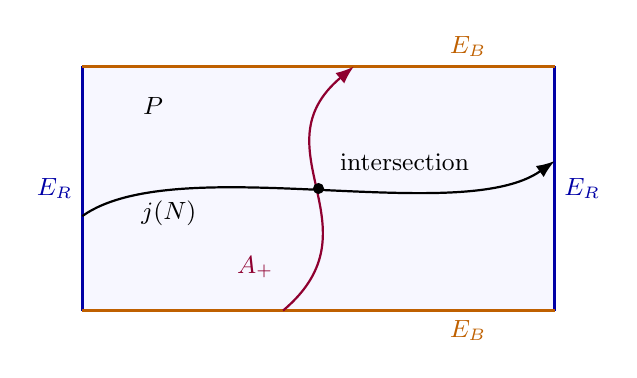
\begin{tikzpicture}[x=1cm,y=1cm,>=Latex,font=\small]
 \fill[blue!3] (-3,-1.55) rectangle (3,1.55);
 \draw[very thick,blue!65!black] (-3,-1.55)--(-3,1.55);
 \draw[very thick,blue!65!black] (3,-1.55)--(3,1.55);
 \draw[very thick,orange!75!black] (-3,-1.55)--(3,-1.55);
 \draw[very thick,orange!75!black] (-3,1.55)--(3,1.55);
 \draw[thick,->] (-3,-.35) .. controls (-1.8,.5) and (1.8,-.5) .. (3,.35);
 \draw[thick,->,purple!75!black] (-.45,-1.55) .. controls (.8,-.5) and (-.8,.5) .. (.45,1.55);
 \fill (0,0) circle (2pt);
 \node[above right] at (.15,.1) {intersection};
 \node[below] at (-1.9,-.03) {$j(N)$};
 \node[left,purple!75!black] at (-.45,-1) {$A_+$};
 \node[left,blue!65!black] at (-3,0) {$E_R$};
 \node[right,blue!65!black] at (3,0) {$E_R$};
 \node[above,orange!75!black] at (1.9,1.55) {$E_B$};
 \node[below,orange!75!black] at (1.9,-1.55) {$E_B$};
 \node at (-2.1,1.05) {$P$};
\end{tikzpicture}
\caption{A schematic transverse section of the compact triad.
The relative cycle $j(N)$ has boundary on the radial side $E_R$ and avoids
$E_B$. Its dual representative $A_+$ has boundary on $E_B$ and is pushed
off $E_R$. Their nonzero intersection becomes a local degree after the
parameter is pulled back and doubled. The drawing records incidence and
boundary conditions, not the dimensions of the cycles.}
\label{fig:degree-triad}
\end{figure}


\begin{proof}[Proof of \cref{thm:comparison-data}]
Double $A_+$ along its boundary, reversing the orientation on the
second copy, to obtain a closed oriented manifold $A$.  Reflect both
component maps $o_0,y_0$ across the seam.  The collar conclusion of
\cref{lem:relative-degree} makes the resulting maps smooth.  Pull back
$\widehat C\to C$ by $o_0:A\to C$, obtaining $\widehat A\to A$, and
form
\[
 Z=X\times_C A=(\widetilde M\times\widehat A)/\Gamma.
\]
The projection $X\to C$ is a submersion, so $Z$ is a smooth
$q$-manifold even though $o_0$ need not be a submersion.  Local sheet
trivializations identify it with a product of the
$\widetilde M$ fibre directions and the $A$ directions, with their product
orientation.  This also exhibits it as the stated cover of $M\times A$.
Continue to write $\mathcal V$ for the pulled-back profile map.

Choose once and for all a smooth function $\eta:[0,\infty)\to[0,1]$
equal to one on $[0,2]$ and zero on $[3,\infty)$, and define
\begin{equation}
\label{eq:comparison-map}
 G=\eta\bigl(\norm{\mathcal V}_{p_R}/T_0\bigr)
       \frac{\mathcal V-y_0}{R}.
\end{equation}
Properness of the profile map and compactness of $A$ imply that its
support is compact.  It is smooth, including at $\mathcal V=0$,
because the cutoff is constant in a neighborhood of that locus.
Write $a:Z\to A$ for the parameter projection, and let
\[
 \Omega=\{z\in Z:\ a(z)\in\operatorname{int}A_+,
                       \norm{\mathcal V(z)}_{p_R}<2T_0\}.
\]
This is relatively compact.  On its angular boundary the defining
boundary inequality for $A_+$ gives
$\norm{\mathcal V-y_0}_\infty>4R$.  On its other boundary,
\[
 \norm{\mathcal V-y_0}_{p_R}
 \ge2T_0-\norm{y_0}_{p_R}>T_0,
\]
and hence $\norm{\mathcal V-y_0}_\infty>T_0/3$.
The cutoff equals one on both parts of the boundary.  In view of
$T_0>100L=10000R$, these bounds prove the boundary assertion in
\cref{eq:comparison-degree}.

The zeros in $\Omega$ are exactly the intersections furnished by
\cref{lem:relative-degree}: if $\mathcal V=y_0$, their common
$p_R$-norm is less than $T_0$, so the point belongs to $N$.
We check orientations to identify their signed count.  In oriented
local lifts, the difference of the two map differentials, in tangent
variables $(v_M,v_C,v_A)$ and target rows $(C,\R^q)$, is
\[
 \begin{pmatrix}
  0&I&-do_0\\
  d_{\widetilde M}\mathcal V&d_C\mathcal V&-dy_0
 \end{pmatrix}.
\]
Substitute $v_C=v'_C+do_0(v_A)$.  This substitution has determinant
one.  Moving the $C$ variables to the front introduces only the fixed
dimensional sign $(-1)^{nd}$, and eliminating their identity block
leaves the differential of the pulled-back $\mathcal V-y_0$ on $Z$.
Thus the intersection signs agree with its zero signs up to one
fixed sign, independent of the point, sheet, and component.  Division
by the positive number $R$ does not change them.  Their nonzero sum
is therefore $\deg(G,\Omega,0)$ up to that sign.  Doubling the parameter
may cancel a global intersection count between its two copies; it
does not change the local degree over the first copy used here.

It remains to check the derivative bound.  By
\cref{lem:distance-profiles,eq:profile-norms},
\[
 \abs{d_{\widetilde M}\mathcal V_i}\le K_0,
 \qquad
 \abs{d_{\widetilde M}\norm{\mathcal V}_{p_R}}\le3K_0
 \quad(\mathcal V\ne0).
\]
In the cutoff transition region,
$\norm{\mathcal V-y_0}_\infty<4T_0$.  Writing
$E_\eta=\sup\abs{\eta'}$, differentiation of
\cref{eq:comparison-map} gives for every row
\[
 \abs{d_{\widetilde M}G_i}
 \le\frac{K_0}{R}
       +\frac{3K_0E_\eta}{T_0}\frac{4T_0}{R}
 \le\frac{K_0(1+12E_\eta)}{R}.
\]
The estimate also holds where the cutoff is constant.  Together with
\cref{eq:profile-count}, it proves \cref{eq:comparison-bounds} with
$J=\max\{J_1,K_0(1+12E_\eta),1\}$, increasing $R_0$ if necessary.
Finally $G$ is a smooth compactly supported map on the lifted product
geometry of the cover $Z\to M\times A$; each of its covariant
derivatives therefore has finite supremum for this fixed $R$.
\end{proof}

\section{A scalar-curvature identity for graph stabilization}
\label{sec:graph-calculus}

One shortening step increases a metric in the direction of a single
function's differential and adds one circle. The circle warp compensates
for the scalar terms introduced by the graph. Warped-circle formulas are
also central to the stabilization used in minimal slicing
\cite[Lemma~2.5]{SchoenYau2017}; here we compute their combination with a
rank-one graph change before choosing the graph by a nonlinear equation.

We use the Laplacian $\Delta=\diver\nabla$ and the convention for which
round spheres have positive scalar curvature. The base $(B,g)$ may have
any finite dimension and may already contain warped circle factors. All
derivatives not explicitly assigned another metric are taken with respect
to $g$.

Let $f\in C^\infty(B)$ and let $N:[0,\infty)\to(0,\infty)$ be smooth and constant near zero. Set
\begin{equation}\label{eq:graph-quantities}
 \begin{gathered}
 t=\abs{df}_g,\qquad W=(1+N(t)^2t^2)^{1/2},\qquad v=W^{-1},\\
 U=vN(t)\nabla f,\qquad r=\abs{U}_g=vN(t)t,\qquad
 D=-\diver_g U.
 \end{gathered}
\end{equation}
Although $t$ and $r$ need not be smooth where $df=0$, the functions $N(t)$
and $v$ and the vector field $U$ are smooth there. Indeed, $N(t)$ is
constant near such points, and the other two are smooth functions of $df$.
We use identities involving $\log t$ or $\log r$ only where $t>0$; the
resulting scalar estimates extend by continuity. Consider
\begin{equation}\label{eq:graph-metric-update}
 g^+=g+N(t)^2df^2+v^2d\theta^2
 \quad\text{on }B\times\T.
\end{equation}
The first two terms form the metric induced on the graph of $f$ in
$(B\times\R,g+N(t)^2dz^2)$, where $N(t)$ is regarded as a fixed function of the base point, independent of $z$.

\begin{proposition}[Exact scalar-curvature identity]\label{prop:scalar-update}
At a point where $t>0$, choose a $g$-orthonormal frame
$e_1=\nabla f/t,e_2,\ldots,e_{\dim B}$, and put
\[
 \mathfrak p=\frac{tN'(t)}{N(t)},\qquad
 A=d\log t,\qquad
 C_{jk}=t^{-1}\Hess_g f(e_j,e_k)\quad(j,k>1).
\]
Then
\begin{equation}\label{eq:scalar-exact}
 \begin{split}
 \Scal_{g^+}-\Scal_g
 ={}&D^2-2U(D)+r^2\abs{C}^2+(e_1r)^2\\
 &+2r^2(1+\mathfrak p)(v^2-\mathfrak p r^2)
       \sum_{j>1}A(e_j)^2.
 \end{split}
\end{equation}
In particular, the final term is nonnegative whenever
$\mathfrak p\ge0$ and $\mathfrak p N(t)^2t^2\le1$.
For $N\equiv1$, one also has, everywhere,
\begin{equation}\label{eq:ordinary-scalar-update}
 \Scal_{g^+}-\Scal_g=\abs{II}^2+D^2-2U(D),
\end{equation}
where $II$ is the second fundamental form of the ordinary product graph.
The inverse graph metric on base covectors and the volume form of $g^+$ are
\begin{equation}\label{eq:graph-inverse-volume}
 P=g^{-1}-U\otimes U,
 \qquad dV_{g^+}=dV_g\,d\theta.
\end{equation}
\end{proposition}

\begin{proof}
Write $E=N^{-1}\partial_z$ and give the graph the upward unit normal
$\nu=-U+vE$. Our convention for the second fundamental form is
$II(X,Y)=\ip{\nabla_X\nu,Y}$, so its trace is
\begin{equation}\label{eq:graph-mean-curvature}
 H=D-U(\log N).
\end{equation}
The vertical Killing field $\partial_z$ has normal speed $Nv$ along the
graph, and its tangential part projects to $NvU$ on the base. Vertical
translation preserves the graph's mean curvature as a function of that
base point. The normal and tangential variation terms must therefore
cancel, giving
\begin{equation}\label{eq:graph-jacobi}
 \bigl(\Delta_{\rm gr}+\abs{II}^2+\Ric_{\rm amb}(\nu,\nu)\bigr)(Nv)
       =Nv\,U(H).
\end{equation}
Here a normal variation of speed $\psi$ changes $H$ by the negative of the
Jacobi operator applied to $\psi$, while a tangential variation
differentiates $H$ in its tangential direction. This fixes the sign on the
right of \eqref{eq:graph-jacobi}.

The classical warped-product formulas \cite[Section~7]{BishopONeill1969},
together with the Gauss equation, give, respectively,
\[
 \begin{aligned}
 \Scal_{\rm amb}&=\Scal_g-2\Delta_gN/N,\\
 \Scal_{\rm gr}&=\Scal_{\rm amb}-2\Ric_{\rm amb}(\nu,\nu)
                         +H^2-\abs{II}^2,\\
 \Scal_{g^+}&=\Scal_{\rm gr}-2\Delta_{\rm gr}v/v.
 \end{aligned}
\]
Expanding $\Delta_{\rm gr}(Nv)$ in \eqref{eq:graph-jacobi} therefore yields
\begin{equation}\label{eq:scalar-before-cancellation}
 \begin{split}
 \Scal_{g^+}-\Scal_g
 ={}&\abs{II}^2+H^2-2U(H)\\
 &+2\frac{(\Delta_{\rm gr}-\Delta_g)N}{N}
   +4\ip{d\log N,d\log v}_{P}.
 \end{split}
\end{equation}
The formula for $P$ in \eqref{eq:graph-inverse-volume} follows directly by inverting the rank-one addition $g+N^2df^2$.

Put $b_0=d\log N$. For a function on the base,
$\Delta_{\rm gr}N$ is its ambient Hessian traced over the graph, minus $H\nu(N)$. Since
$\Hess_{\rm amb}N(E,E)=N\abs{b_0}^2$, this gives
\begin{equation}\label{eq:graph-laplacian-correction}
 \frac{(\Delta_{\rm gr}-\Delta_g)N}{N}
 =-\Hess_g\log N(U,U)-b_0(U)^2
       +r^2\abs{b_0}^2+H b_0(U).
\end{equation}
Substitute $H=D-b_0(U)$ in \eqref{eq:scalar-before-cancellation}. The Hessian terms cancel because
\[
 U\bigl(b_0(U)\bigr)
   =\Hess_g\log N(U,U)+b_0(\nabla^g_UU).
\]
The result is
\begin{equation}\label{eq:scalar-intermediate}
 \begin{split}
 \Scal_{g^+}-\Scal_g
 ={}&\abs{II}^2+D^2-2U(D)
       +2b_0(\nabla^g_UU)-3b_0(U)^2\\
 &+2r^2\abs{b_0}^2+4\ip{b_0,d\log v}_{P}.
 \end{split}
\end{equation}
When $N\equiv1$, all terms involving $b_0$ vanish. This proves
\eqref{eq:ordinary-scalar-update} without any condition on $D$ other than its definition.

For the remaining calculation use the graph-orthonormal frame
$T=ve_1+rE,e_2,\ldots,e_{\dim B}$. For base vector fields lifted independently of $z$, the ambient connection satisfies
\[
 \nabla_X^{\rm amb}E=0,\qquad
 \nabla_E^{\rm amb}X=b_0(X)E,\qquad
 \nabla_E^{\rm amb}E=-b_0^{\sharp}.
\]
Differentiating $\nu=-U+vE$ gives
\begin{equation}\label{eq:graph-second-form}
 \begin{aligned}
 II(T,T)&=-r\bigl[v^2(1+\mathfrak p)+\mathfrak p\bigr]A(e_1),\\
 II(T,e_j)&=-rv(1+\mathfrak p)A(e_j),\qquad j>1,\\
 II(e_j,e_k)&=-rC_{jk},\qquad j,k>1.
 \end{aligned}
\end{equation}
Moreover,
\begin{equation}\label{eq:graph-log-derivatives}
 \begin{gathered}
 b_0=\mathfrak p A,\qquad
 d\log r=v^2(1+\mathfrak p)A,\qquad
 d\log v=-r^2(1+\mathfrak p)A,\\
 \nabla^g_UU=r^2\left(v^2(1+\mathfrak p)A(e_1)e_1
                         +\sum_{j>1}A(e_j)e_j\right).
 \end{gathered}
\end{equation}
For the last equality, symmetry of $\Hess f$ gives
$\nabla_{e_1}e_1=\sum_{j>1}A(e_j)e_j$.

After substitution in \eqref{eq:scalar-intermediate}, the $C$ terms give
$r^2\abs{C}^2$. The remaining terms are squares of the component of $A$
along $e_1$ and of its components orthogonal to $e_1$. After division by
$r^2$, the coefficient of $A(e_1)^2$ is
\[
 \begin{split}
 &\bigl[v^2(1+\mathfrak p)+\mathfrak p\bigr]^2
       -2\mathfrak p v^2(1+\mathfrak p)-\mathfrak p^2\\
 &\hspace{35mm}=v^4(1+\mathfrak p)^2.
 \end{split}
\]
For every $j>1$, the corresponding coefficient is
\[
 2v^2(1+\mathfrak p)^2-2\mathfrak p(1+\mathfrak p)
       =2(1+\mathfrak p)(v^2-\mathfrak p r^2).
\]
Since $e_1r=rv^2(1+\mathfrak p)A(e_1)$, these are precisely
\eqref{eq:scalar-exact}. Also
\[
 v^2-\mathfrak p r^2=v^2\bigl(1-\mathfrak p N(t)^2t^2\bigr),
\]
which proves the positivity assertion. Finally,
$\det(g+N^2df^2)=W^2\det g$ and $vW=1$ prove the volume identity.
\end{proof}

The inverse-metric decrease will later let us sum the costs of many graph
changes in a fixed $n$-dimensional space. First we must choose each graph
so that the remaining term $D^2-2U(D)$ can be bounded from below.
The next section proves existence for the equation used for this choice.

\section{Solving the graph equation on a cover}
\label{sec:graph-existence}

The scalar identity alone does not construct a graph. We now solve a
nonlinear equation prescribing its divergence in terms of the error from
a given function. The strict tangent band controls that error, while
uniqueness will allow the solutions to descend through the flat-bundle
transition maps and remain invariant under previously added circles.

The graph regularization and gradient-estimate strategy was inspired by
the Jang-equation capillarity method of Schoen--Yau
\cite[Section~4, pp.~251--253]{SchoenYau1981}.  The variable flux, tangent
forcing, stabilization identity, and fixed-rank shortening estimates
needed here are developed in this paper; their existence theorem is not
being applied to the present equation.

We specify the uniformity needed for the nonlinear equation. Let $B$ be a Riemannian cover of a closed manifold, with lifted reference metric $g_{\rm ref}$. Fix nested coordinate charts obtained by lifting a finite collection of relatively compact reference charts, with the smaller charts covering $B$. For $0<\alpha<1$, uniform $C^{j,\alpha}$ norms are the suprema of the usual chart norms on these smaller charts; the larger charts provide room for interior estimates. Equivalent choices give equivalent norms. A metric $g$ is \emph{uniformly controlled} if it is uniformly equivalent to $g_{\rm ref}$ and its coordinate coefficients have bounded derivatives of every order. The metric need not be invariant under deck transformations. We write $C_b^{j,\alpha}$ for these uniform H\"older spaces and $C_b^\infty$ for smooth functions with bounded derivatives of every order.

Products of such covers with any fixed finite torus have the same properties. In all assertions in this Section, constants may depend on the particular finite-dimensional geometry and the fixed equation coefficients.

\begin{lemma}[A uniform linear inverse]\label{lem:uniform-linear}
Suppose that, in the reference charts, a scalar operator has the form
\[
 L\xi=-a^{ij}\partial_i\partial_j\xi+b^i\partial_i\xi+c\xi,
\]
with uniformly $C^{0,\alpha}$ coefficients, uniformly bounded drift, uniformly positive definite principal matrix, and $c\ge c_0>0$. Then
\[
 L:C_b^{2,\alpha}(B)\longrightarrow C_b^{0,\alpha}(B)
\]
is an isomorphism. Its inverse is bounded in terms of the indicated uniform bounds. If the coefficients have bounded derivatives of every order, the inverse also maps $C_b^{j,\alpha}$ boundedly into $C_b^{j+2,\alpha}$ for every $j\ge0$.
\end{lemma}

\begin{proof}
It suffices to prove the assertion when $\dim B\ge2$. If $d=\dim B<2$,
put $T_0=\T^{2-d}$ with its flat product metric and consider
$\overline L=L-\Delta_{T_0}$ on $B\times T_0$, with right-hand side
pulled back from $B$. Its principal matrix is uniformly positive and its
zeroth-order coefficient is still at least $c_0$. The result in dimension
two gives a unique solution; translation invariance of the data and
uniqueness make that solution independent of $T_0$. It therefore descends
to the required solution on $B$. Restriction to a fixed torus point gives
the same uniform estimates, and lifting two possible solutions proves
uniqueness on $B$.

Take a smooth compact exhaustion and solve the zero-boundary Dirichlet problem on each member. Bounded-domain elliptic Dirichlet theory applies since the principal matrix is uniformly positive and the zeroth-order term has the indicated sign; see, for example, the linear Schauder theory in \cite[Theorems~6.2 and~6.14]{GilbargTrudinger2001}. The maximum principle gives, for right-hand side $F$,
\begin{equation}\label{eq:uniform-inverse-sup}
 \norm{\xi}_{\infty}\le c_0^{-1}\norm{F}_{\infty},
\end{equation}
independently of the exhaustion domain. On every smaller reference chart whose enlargement is contained in that domain, the interior estimate gives
\[
 \norm{\xi}_{C^{2,\alpha}(\text{smaller chart})}
 \le C\bigl(\norm{F}_{C^{0,\alpha}(\text{larger chart})}
                         +\norm{\xi}_{\infty}\bigr),
\]
with one constant for all charts. Local compactness and a diagonal subsequence produce a solution on $B$. Each fixed enlarged chart eventually lies in the exhaustion, so the same estimate holds at every point of the limit. Taking the supremum over charts proves that the solution belongs to $C_b^{2,\alpha}$ with a bounded norm. No estimate at the moving exhaustion boundary is needed. If $B$ is compact, one instead uses the closed-manifold version of the same theory.

For uniqueness, suppose $L\xi=0$ and $S=\sup_B\xi>0$. Center uniform charts at a sequence of points where $\xi\to S$. The pulled-back coefficients have a convergent local $C^{0,\beta}$ subsequence, and the functions a convergent $C^{2,\beta}$ subsequence, for $0<\beta<\alpha$. At the center of the limiting chart the limiting function attains the maximum $S$. There its gradient vanishes and its Hessian is negative semidefinite, so
\[
 L\xi\ge c_0S>0,
\]
a contradiction. Apply the same argument to $-\xi$. This also proves the global maximum principle used in \eqref{eq:uniform-inverse-sup} for any solution in the uniform class. Higher-order interior estimates give the final assertion.
\end{proof}

\begin{theorem}[Uniform graph solvability]\label{thm:uniform-graph}
Let $(B,g)$ be uniformly controlled as above, and let $\ell\in C_b^\infty(B)$. Fix $\eps,w,B_0,s>0$ and $0\le\beta<1$. Suppose $N$ is smooth, positive, nondecreasing, constant near zero, and equal to $1$ for $t\ge1/2$. Define the quantities in \eqref{eq:graph-quantities} and
\[
 \lambda(r)=B_0(r^2+s^2)^{\beta/2}.
\]
There is a unique solution in the uniform $C^{2,\alpha}$ class with a uniform band margin to
\begin{equation}\label{eq:graph-equation}
 -\diver_g U
   =\lambda(r)\tan\left(\frac{\ell-\eps f}{w}\right),
 \qquad \abs{\ell-\eps f}<\frac{\pi w}{2}.
\end{equation}
This solution lies in $C_b^\infty(B)$, and the band has a positive uniform margin.
The metric \eqref{eq:graph-metric-update} is uniformly controlled and complete.

The solution is invariant under every isometry preserving the equation's
data. The following parameter statement will be used below. Fix the
reference cover, its metric and nested charts, and the equation parameters
$\eps,w,B_0,s,\beta,N$. Let $(g_a,\ell_a)$ be a jointly smooth family over
a finite-dimensional parameter manifold $A$. For every relatively compact
subset $V'\Subset V$ of a parameter chart, assume common constants
$c_{V'},C_{V'}>0$ such that
\[
 c_{V'}g_{\rm ref}\le g_a\le C_{V'}g_{\rm ref}\qquad(a\in V'),
\]
and common bounds in the fixed reference charts for every mixed derivative
of the coefficients of $g_a$ and of $\ell_a$, including order zero. Then
$a\mapsto f_a$ is smooth in every $C_b^{j,\alpha}$ norm, for $j\ge0$ and
$0<\alpha<1$. If $A$ is compact,
all mixed derivatives of $f_a$ are uniformly bounded and the tangent band
has a common positive margin. For a bundle of such covers, the local
solutions glue whenever fixed reference deck transformations carry one
local data set to another.
\end{theorem}

\begin{proof}
We may assume $\dim B\ge2$. Once the theorem is proved in those dimensions,
the lower-dimensional cases follow by taking the product with
$T_0=\T^{2-\dim B}$, using the product metric and pulling back $\ell$.
The solution on $B\times T_0$ is invariant under $T_0$ translations by
uniqueness, and hence is pulled back from a function on $B$. For such a
function the flux is $(U,0)$ and its product divergence is $\diver_g U$,
so the descended function solves exactly \eqref{eq:graph-equation}.
Restriction to a fixed torus point gives the uniform and parameter bounds,
and lifting two possible solutions gives uniqueness. The graph metric
claims then follow from the same final bounds below.

Replace $\ell$ by $\tau\ell$, $0\le\tau\le1$, and start at $f=0$ for $\tau=0$. We use $C_b^{2,\alpha}(B)$, for a fixed $0<\alpha<1$, as the solution space.

\smallskip\noindent\textbf{Linearization and openness.}
As a function of the covector $df$, the flux $U$ has transverse eigenvalue $r(t)/t$ and radial eigenvalue
\begin{equation}\label{eq:graph-flux-ellipticity}
 r'(t)=\frac{N(t)(1+\mathfrak p(t))}
                {(1+N(t)^2t^2)^{3/2}}>0.
\end{equation}
Both extend positively and smoothly through $t=0$, since $N$ is constant there. Hence the equation is uniformly elliptic on every bounded gradient range.

On the open set of $C_b^{2,\alpha}$ functions with a positive uniform margin in the tangent band, the equation is a smooth map into $C_b^{0,\alpha}$. The apparent nonsmoothness of $r=\abs{U}$ at zero causes no problem: $\lambda$ is a smooth function of $r^2$, and the flux is smooth in $df$. At an individual solution, moving the right-hand side to the left gives the linearization
\begin{equation}\label{eq:graph-linearization}
 -\diver_g\bigl(a_f(d\xi)\bigr)+\mathbf b(d\xi)
   +\frac{\eps\lambda(r)}w
       \sec^2\left(\frac{\tau\ell-\eps f}{w}\right)\xi.
\end{equation}
Here $a_f$ is the derivative of the flux. After expansion, the coefficients are uniformly H\"older, and the zeroth-order coefficient is at least
$\eps B_0s^\beta/w>0$. The individual $C_b^{2,\alpha}$ bound supplies a bounded gradient range, so \cref{lem:uniform-linear} makes the linearization invertible. The Banach implicit function theorem proves openness in $\tau$.

\smallskip\noindent\textbf{Comparison and individual regularity.}
Two solutions in this class agree. To see this, take a positive supremum of their difference, if one exists, and pass to a limiting uniform chart as in \cref{lem:uniform-linear}. At the limiting maximum their gradients agree and their Hessians are ordered. At that common gradient the right-hand side of the equation is strictly decreasing in height, with derivative at most $-\eps B_0s^\beta/w$. The two equations are therefore incompatible. The same argument compares a solution with a strict upper or lower barrier.

Each individual solution has uniform bounds in every higher derivative before we seek bounds independent of $\tau$. Indeed its given $C_b^{2,\alpha}$ norm and band margin make the equation uniformly elliptic with smooth nonlinearities on a bounded range. In a chart, write its nondivergence form as
\[
 a^{ij}(x,df)f_{ij}=H(x,f,df).
\]
For $z=\partial_k f$, differentiation, initially by difference quotients, gives
\begin{equation}\label{eq:individual-graph-bootstrap}
 \begin{split}
 a^{ij}\partial_i\partial_j z
  +\bigl(a^{ij}_{p_l}f_{ij}-H_{p_l}\bigr)\partial_lz-H_fz
   =H_{x_k}-a^{ij}_{x_k}f_{ij}.
 \end{split}
\end{equation}
The coefficients and source are uniformly $C^{0,\alpha}$ using only the individual $C^{2,\alpha}$ bound. The difference quotients have bounded sup norms, so interior Schauder estimates on smaller charts give $f\in C_b^{3,\alpha}$. Iterating gives $C_b^\infty$. These constants may at this stage depend on the individual solution.

\smallskip\noindent\textbf{Uniform tangent-band barriers.}
For $\delta>0$ consider
\[
 f_\pm=\eps^{-1}\bigl(\tau\ell\pm(\pi/2-\delta)w\bigr).
\]
Their gradient and divergence terms are bounded uniformly in $\tau$ and in small $\delta$. At $f_+$ the tangent term is negative and diverges uniformly to $-\infty$ as $\delta\downarrow0$; at $f_-$ it diverges uniformly to $+\infty$. This uses $\lambda\ge B_0s^\beta>0$. Choose a sufficiently small fixed $\delta$ so that these are strict upper and lower barriers. Comparison gives, for every solution along the homotopy,
\begin{equation}\label{eq:uniform-graph-band}
 f_-\le f\le f_+,
 \qquad
 \abs{\tau\ell-\eps f}\le(\pi/2-\delta)w.
\end{equation}
In particular the heights and the band margins are now controlled independently of $\tau$.

\smallskip\noindent\textbf{A uniform gradient bound.}
Fix one solution along the continuation path. If $\sup_B t\le1$, there is
nothing to prove. Otherwise choose points where $t$ approaches its
supremum. The individual higher bounds just established allow the metric,
data, and solution to converge in uniform charts, in enough derivatives
for the graph equation and its Jacobi identity. The limiting slope attains
its maximum at the center. This passage uses finite bounds for that one
solution; the estimate obtained at the maximum will depend only on the
fixed data and the uniform band margin.

At this maximum, $t>1$, so $N=1$ on a neighborhood. The graph is locally an ordinary product graph, $v=(1+t^2)^{-1/2}$ has a minimum, and $dr=0$. Put
\[
 h_e=\frac1w\left(\lambda+\frac{D^2}{\lambda}\right)
     =\frac{\lambda}{w}
          \sec^2\left(\frac{\tau\ell-\eps f}{w}\right).
\]
Differentiating the right-hand side of the equation along $U$, and using $dr=0$ and $vU(f)=r^2$, the vertical translation identity becomes
\begin{equation}\label{eq:gradient-jacobi}
 \bigl(\Delta_{\rm gr}+\abs{II}^2+\Ric_{g+dz^2}(\nu,\nu)\bigr)v
       =v h_e\tau U(\ell)-\eps h_e r^2.
\end{equation}
The band bound implies fixed constants $0<h_{\min}\le h_e\le h_{\max}<\infty$. The fixed uniformly controlled base has $\Ric_g\ge-C_{\rm Ric}g$. At the minimum of $v$, the left-hand side of \eqref{eq:gradient-jacobi} is at least $-C_{\rm Ric}v$. Since $r^2>1/2$ there and $\abs{U(\ell)}\le\norm{d\ell}_{\infty}$, it follows that
\[
 \frac{\eps h_{\min}}2
 \le v\bigl(C_{\rm Ric}+h_{\max}\norm{d\ell}_{\infty}\bigr).
\]
This bounds $v$ below by a positive constant and hence bounds $t$ above, uniformly in $\tau$. One may add $1$ to the denominator when writing an explicit positive bound. All constants in this final estimate depend only on the fixed data and the already uniform band margin; the individual higher norms used to attain the limiting maximum have disappeared.

\smallskip\noindent\textbf{Uniform higher estimates and closedness.}
After the gradient estimate, the flux is uniformly elliptic on a fixed bounded range. Absorbing the metric volume density, write
\[
 -\partial_i\mathcal A^i(x,\partial f)
       =\mathcal H(x,f,\partial f).
\]
Every coordinate derivative $z=\partial_k f$ satisfies
\begin{equation}\label{eq:graph-divergence-bootstrap}
 -\partial_i\bigl(\mathcal A^i_{p_j}\partial_jz\bigr)
  =\mathcal H_{p_j}\partial_jz+\mathcal H_f z+\mathcal H_{x_k}
       +\partial_i\mathcal A^i_{x_k}.
\end{equation}
The drift coefficient and the nondivergence source are uniformly bounded;
the last term is the divergence of a uniformly bounded vector field.
Interior H\"older regularity for scalar divergence-form equations gives a
uniform $C^{0,\alpha'}$ bound for $z$ on smaller charts, for some
$\alpha'>0$; we use \cite[Theorem~8.24]{GilbargTrudinger2001}. In that
theorem's notation take $b^i=d=0$, retain the bounded drift, and treat
$\mathcal H_fz+\mathcal H_{x_k}$ as scalar data and $\mathcal A^i_{x_k}$ as
divergence data, with the signs determined by
\eqref{eq:graph-divergence-bootstrap}. On a fixed chart these bounded data
satisfy its $L^{r/2}$ and $L^r$ hypotheses for any finite $r>\dim B$.
The estimate uses the local $L^2$ norm of $z$, already controlled by the
gradient bound; it requires no bound for the derivatives of $z$. Thus its
constants depend only on ellipticity, the fixed chart size, the displayed
data bounds, and the gradient bound. We obtain a uniform
$C^{1,\alpha'}$ bound for $f$.

The original equation now has uniformly $C^{0,\alpha'}$ nondivergence coefficients and right-hand side. Interior Schauder estimates give $C^{2,\alpha'}$ bounds, and \eqref{eq:individual-graph-bootstrap} gives higher uniform bounds by iteration. In particular these imply uniform $C^{2,\alpha}$ bounds for the originally chosen $\alpha<1$, by using a bound on one further derivative. Given a sequence of solvable parameters tending to $\tau_*$, local compactness on an exhaustion produces a solution at $\tau_*$ with the same uniform bounds and band margin. The solvable set is therefore closed as well as open, and contains all of $[0,1]$.

\smallskip\noindent\textbf{Symmetries and parameter dependence.}
An isometry preserving the data takes a solution to a solution; uniqueness
gives invariance. More generally, an isometry carrying one set of data to
another carries their solutions to one another by pullback. The uniform
solution class is preserved: covariant H\"older norms for the uniformly
controlled metric are equivalent to the reference-chart norms, and these
intrinsic norms are unchanged under an isometry. In particular all old torus translations preserve a solution when they preserve the input data.

For parameter dependence it is essential to use the stated mixed bounds. If $h(x,a)$ is any input coefficient in a local parameter chart, bounds on its mixed derivatives imply smoothness of $a\mapsto h(\cdot,a)$ in every $C_b^{j,\alpha}$ norm. Explicitly, Taylor's formula in $a$, applied also to $x$ derivatives through order $j+1$, gives
\[
 \norm{h(\cdot,a+u)-h(\cdot,a)-D_a h(\cdot,a)u}_{C_b^{j,\alpha}}
       \le C\abs{u}^2.
\]
The additional $x$ derivative controls the H\"older seminorm on the uniformly bounded charts. Applying the same argument to every parameter derivative proves the claimed Banach-space smoothness.

The equation is therefore a smooth Banach map in $a$ as well as $f$.
The fixed reference charts supply the Banach spaces, while the common
metric equivalence on $V'$ supplies locally uniform ellipticity on bounded
gradient ranges. At each parameter,
the invertible linearization gives a locally smooth solution by the
implicit function theorem. Applying the higher-order part of
\cref{lem:uniform-linear} gives the same conclusion in every higher norm,
and uniqueness identifies all the local branches. Compactness of $A$
supplies uniform mixed bounds and a common band margin using finitely many
such neighborhoods.

For gluing, suppose a fixed reference deck transformation $\psi$ carries
one local data set to another, so that
$g_a^{(2)}=\psi^*g_a^{(1)}$ and $\ell_a^{(2)}=\psi^*\ell_a^{(1)}$.
It is then an isometry between those data sets. Naturality and uniqueness
give $f_a^{(2)}=\psi^*f_a^{(1)}$. Extending $\psi$ by the identity on old
circle factors gives the compatibility needed for the flat bundles below.

Finally, $df$ is bounded, $N$ is positive and bounded on its attained range, and $v$ is bounded below. Thus $g^+$ is uniformly equivalent to the reference product metric and has bounded coefficient derivatives of every order. Its completeness follows from that equivalence to a complete reference metric.
\end{proof}

We have obtained a smooth graph for each fixed finite set of data, together
with the symmetry and parameter control needed to repeat the construction.
The estimates in the next section will use its equation to bound scalar
loss independently of these potentially large analytic regularity constants.

\section{Shortening all comparison coordinates}
\label{sec:shortening}

Return to the flat bundle
\[
 Z=(\widetilde M\times\widehat A)/\Gamma\longrightarrow A,
 \qquad q=n+\dim A,
\]
where $M^n$ and $A$ are closed and $\widehat A\to A$ is a principal left
$\Gamma$-cover. The covering projection to $M\times A$ induces the splitting
$TZ=E_M\oplus E_A$ described in \cref{thm:comparison-data}. Here $E_M$ is
tangent to the $\widetilde M$ fibres, while $E_A$ is the flat lift of the
parameter directions. Local choices of sheets over $A$ identify the fibres
with $\widetilde M$; the transition maps are fixed deck transformations.
We first change the metric in the fibre directions and add circles. The
metric on $E_A$ is introduced only in the final assembly step.

A metric with $b$ stabilizing circles has, locally over $A$, the form
\begin{equation}\label{eq:fibre-stabilized-metric}
 g_h(x,a)+\sum_{\nu=1}^b m_\nu(x,a)^2d\theta_\nu^2.
\end{equation}
Here $g_h$ acts on the $n$ fibre directions, the positive warps depend only on $x,a$, and the metric is invariant under all circle translations. At every fixed finite stage, the coefficients and all mixed derivatives will be bounded, and the metric will be uniformly equivalent to the lifted reference product. These bounds may depend on the stage.

Until the parameter metric is assembled in
\cref{lem:parameter-scaling}, every differential, gradient and scalar
curvature is computed on the fibre $\widetilde M\times\T^b$ with
$a\in A$ fixed. The functions and metrics may vary smoothly with $a$;
this variation is measured separately by the mixed derivative bounds.
Thus a torus-invariant fibre differential lies in the original $n$
fibre directions, even though its full differential on $Z$ may
have a nonzero parameter component.

\subsection{The cost of one pass}

A pass processes each of $q$ comparison functions once. In this section,
$L$ denotes a bound for their current fibre differentials. The scalar
estimate for a pass depends on $n$ and $\log q$, even though the full fibre
dimension includes all the circles already introduced.

\begin{lemma}[One pass]\label{lem:one-pass}
Let $q\ge2$ and $L,w>0$. On a uniformly controlled metric of the form
\eqref{eq:fibre-stabilized-metric}, suppose smooth bounded torus-invariant
functions $\ell_1,\ldots,\ell_q$ have bounded derivatives of every order.
For a smooth family over a compact parameter manifold, assume in each of
finitely many parameter charts common bounds for every mixed fibre and
parameter derivative of the metric coefficients, warps, and functions,
and a common equivalence to the reference fibre product. Suppose
\[
 \abs{d\ell_i}_{g_*}\le L,
\]
where $g_*$ denotes the metric on $E_M$ at the start of the pass. Then one
can add $q$ circles and replace these functions by $\ell_i^+$ so that
\begin{equation}\label{eq:pass-function-bounds}
 \abs{\ell_i^+-\ell_i}<\frac\pi2w,
 \qquad \abs{d\ell_i^+}_{g_h^+}\le\frac L4,
 \qquad g_h^+\ge g_*.
\end{equation}
For an absolute constant $C_0$, the full fibre scalar curvature satisfies
\begin{equation}\label{eq:pass-scalar-bound}
 \Scal_{g^+}\ge\Scal_g
       -C_0(n+1)(2+\log q)\frac{L^2}{w^2}.
\end{equation}
All data at the new finite stage remain uniformly controlled. For a compact
parameter family satisfying the stated hypotheses, the new mixed derivatives
are also uniformly bounded.
\end{lemma}

\begin{proof}
Set
\begin{equation}\label{eq:pass-parameters}
 \eps=L/4,\qquad a_0=(2+\log q)^{-1},\qquad
 \beta=1-a_0,\qquad s=q^{-3},\qquad B_0=\frac{4L}{a_0w}.
\end{equation}
Choose a smooth nondecreasing cutoff $\phi$ which is zero for $t\le1/4$, one for $t\ge1/2$, and satisfies $0\le\phi'\le10$. Let
\begin{equation}\label{eq:pass-cutoff}
 N(t)^2=s^2+(1-s^2)\phi(t).
\end{equation}
Writing $\mathfrak p=tN'/N$, we have
\begin{equation}\label{eq:pass-cutoff-positivity}
 \mathfrak p\ge0,\qquad
 \mathfrak p N(t)^2t^2
       =\tfrac12 t^3(1-s^2)\phi'(t)\le5/8<1.
\end{equation}
The expression vanishes outside $[1/4,1/2]$, which justifies the displayed bound.

For one coordinate, denote the original function by $\ell$ and the current full fibre metric by $g$. Solve \eqref{eq:graph-equation} with these choices and replace
\[
 g\longmapsto g^+=g+N(t)^2df^2+v^2d\theta^2,
 \qquad \ell\longmapsto\ell^+=\eps f.
\]
\Cref{thm:uniform-graph} applies on $\widetilde M\times\T^b$. Its
uniqueness gives torus invariance and compatibility with the parameter
trivializations. Consequently $df$ vanishes on the circle directions, so
the metric retains the form \eqref{eq:fibre-stabilized-metric}. Its block
on $E_M$ has only increased. Since
\[
 \abs{df}_{g^+}=vt\le1
\]
(the inequality is immediate for $t<1/2$, and $N=1$ for $t\ge1/2$), the new coordinate has derivative norm at most $L/4$. Subsequent steps can only improve this bound. The tangent band gives the height estimate in \eqref{eq:pass-function-bounds}.

It remains to estimate the scalar loss in a way that can be summed. At $t>0$, put $z=e_1r$. Differentiating $\lambda(r)=B_0(r^2+s^2)^{\beta/2}$ along $U=re_1$ gives
\[
 \frac{U(\lambda)}{\lambda}=\gamma z,
 \qquad \gamma=\frac{\beta r^2}{r^2+s^2}\in[0,\beta].
\]
The part of $-2U(D)$ contributed by this derivative is $-2\gamma zD$. Hence
\begin{equation}\label{eq:pass-square-absorption}
 D^2+z^2-2\gamma zD
       \ge(1-\gamma^2)D^2\ge a_0D^2.
\end{equation}
By \eqref{eq:pass-cutoff-positivity}, the final term of \eqref{eq:scalar-exact} is nonnegative.

Measure the vector $U$ in the metric at the start of the pass, and set
\[
 b_U=\abs{U}_{g_*}.
\]
Since the current metric on $E_M$ is at least $g_*$, one has $b_U\le r$.
The input coordinate still satisfies $\abs{d\ell}_{g_*}\le L$, so
$U(\ell)\le Lb_U$, while $U(f)=rt$. Differentiating the tangent in the
equation therefore contributes an adverse term bounded above by
\begin{equation}\label{eq:pass-adverse-term}
 \frac2w\left(\lambda+\frac{D^2}{\lambda}\right)
                      (Lb_U-\eps rt)_+.
\end{equation}
Since $0\le r<1$ and $\beta<1$,
\[
 \lambda=B_0(r^2+s^2)^{\beta/2}\ge B_0r.
\]
Thus the $D^2$ part of \eqref{eq:pass-adverse-term} is at most
\[
 \frac{2L}{wB_0}D^2=\frac{a_0}{2}D^2,
\]
which is absorbed by \eqref{eq:pass-square-absorption}.

For the remaining part, first suppose $r<s$. Then
\begin{equation}\label{eq:pass-small-slope}
 \lambda b_U\le \sqrt2 B_0s^{\beta+1}\le\frac{\sqrt2 B_0}{q}.
\end{equation}
Here $s=q^{-3}$ and $\beta>0$. If instead $r\ge s$, then $t\ge1/4$: for $t<1/4$ one has $N=s$ and $r< s/4$. On the adverse region where $Lb_U-\eps rt>0$, it follows that
\[
 b_U>\frac{rt}{4}\ge\frac r{16}.
\]
Moreover,
\[
 r^{-a_0}\le s^{-a_0}
       =\exp\left(\frac{3\log q}{2+\log q}\right)\le e^3.
\]
Consequently, on that region,
\begin{equation}\label{eq:pass-large-slope}
 \lambda b_U\le\sqrt2 B_0r^{1-a_0}b_U
            \le16\sqrt2 e^3B_0b_U^2.
\end{equation}
Combining these estimates and substituting $B_0$ from \eqref{eq:pass-parameters} gives the one-coordinate inequality
\begin{equation}\label{eq:coordinate-scalar-cost}
 \Scal_{g^+}\ge\Scal_g
      -C_0\frac{L^2}{a_0w^2}\left(\frac1q+b_U^2\right).
\end{equation}
For example $C_0=128\sqrt2 e^3$ is sufficient. The inequality extends by continuity to the boundary of $\{t>0\}$. On the interior of $\{t=0\}$ the graph is constant and the update adds a constant circle, so it holds there as well.

Finally sum \eqref{eq:coordinate-scalar-cost} over the $q$ coordinates.
At a fixed point of $Z$, the inverse metrics of the $E_M$ blocks all act
on the same $n$-dimensional space $E_M^*$. If $U_i$ is the vector used at the $i$th
step, \eqref{eq:graph-inverse-volume} gives the telescoping identity
\begin{equation}\label{eq:pass-trace-telescope}
 \sum_{i=1}^q U_i\otimes U_i
       =g_*^{-1}-(g_h^+)^{-1}\le g_*^{-1}.
\end{equation}
Taking its $g_*$-trace gives $\sum_i b_{U_i}^2\le n$. The $q$ terms $1/q$ sum to $1$, proving \eqref{eq:pass-scalar-bound}. In particular the growing number of old circle directions does not appear in this trace. Uniform control and smooth parameter dependence at the new stage follow from \cref{thm:uniform-graph} applied successively a finite number of times.
\end{proof}

\subsection{Finite iteration and the parameter directions}

We shall use the following elementary assembly observation.

\begin{lemma}[Magnifying the parameter metric]\label{lem:parameter-scaling}
Fix a finite-stage smooth family of metrics of the form
\eqref{eq:fibre-stabilized-metric}, equivariant under the flat transition maps over the closed manifold $A$, with all mixed derivatives bounded and uniform equivalence to a reference product. For any fixed metric $g_A$ on $A$, set
\[
 g_P=g_h+P^2g_A+\sum_{\nu=1}^b m_\nu^2d\theta_\nu^2
 \quad\text{on }Z\times\T^b,
\]
using the flat splitting and no mixed parameter terms. As $P\to\infty$, $\Scal_{g_P}$ converges uniformly to the scalar curvature of the fibre metrics. If $H:Z\to\R^q$ has bounded mixed derivatives, its differential in the parameter directions has norm tending uniformly to zero. Each $g_P$ is complete and uniformly controlled.
\end{lemma}

\begin{proof}
In a parameter chart about $a_*$ write $a=a_*+P^{-1}y$. The parameter block becomes $g_A(a_*+P^{-1}y)$, and the other metric coefficients are the corresponding fibre coefficients evaluated at $a_*+P^{-1}y$. All parameter derivatives through order two tend uniformly to zero. Their limits, at $y=0$, are the two-jets of the fibre metric with $a=a_*$ frozen, times the constant Euclidean parameter block $g_A(a_*)$. Inverses remain uniformly bounded for this fixed stage. The scalar-curvature formula is a continuous expression in these metric two-jets and their inverses, so its limit is uniformly the fibre scalar curvature. The finitely many parameter charts and the assumed bounds make the convergence uniform over all of $Z$.

The parameter differential of $H$ acquires the factor $P^{-1}$, proving the second assertion. The reference product on $Z$ is the pullback of a metric on the closed manifold $M\times A$ and is complete. The assembled metric, with its finite number of circle blocks, is uniformly equivalent to this complete reference product and has bounded coefficient derivatives.
\end{proof}

\begin{theorem}[Logarithmic shortening]\label{thm:shortening}
Suppose $\Scal_M\ge\kappa>0$. On the above bundle $Z$, let
$G:Z\to\R^q$ be smooth and bounded with all mixed derivatives bounded, and suppose $L_0>0$ and
\[
 \sup_{1\le i\le q}\abs{d_{\widetilde M}G_i}\le L_0,
 \qquad q\ge2.
\]
There is a constant $C_n$ depending only on $n$ such that, if
\begin{equation}\label{eq:shortening-smallness}
 C_n(2+\log q)L_0^2\le\kappa/4,
\end{equation}
then for every finite integer $k\ge1$ there are a complete stabilized metric
\[
 \mathfrak g_k=h_k+\sum_{\nu=1}^{kq}m_{k,\nu}^2d\theta_\nu^2
 \quad\text{on }Z\times\T^{kq}
\]
and a smooth bounded map $G^{(k)}:Z\to\R^q$ satisfying
\begin{equation}\label{eq:shortening-output}
 \Scal_{\mathfrak g_k}\ge\kappa/2,\qquad
 \norm{G^{(k)}-G}_{\infty}<\pi/10,\qquad
 \abs{dG^{(k)}}_{\rm op}\le\sqrt{q+1}\,4^{-k}L_0.
\end{equation}
The infinity norm in the middle inequality is the target coordinate maximum, followed by the supremum over $Z$. All metric coefficients, warps, and maps have uniform bounds of every order at each fixed finite stage; their equivalence and derivative constants may depend on that stage.
\end{theorem}

\begin{proof}
Start with the lifted metric of $M$ and no circles, and perform passes indexed by $j=0,\ldots,k-1$ with
\begin{equation}\label{eq:pass-schedule}
 L_j=4^{-j}L_0,\qquad w_j=2^{-j}/10.
\end{equation}
\Cref{lem:one-pass} applies inductively because every coordinate derivative is divided by at least four in each pass. Every stage is finite, so the uniform control required for its successor follows from the last assertion of that Lemma. All local constructions match under the flat parameter transitions by uniqueness of the graph solution.

For any number of passes, the total scalar loss is at most
\[
 C_0(n+1)(2+\log q)\sum_{j\ge0}\frac{L_j^2}{w_j^2}
   =\frac{400}{3}C_0(n+1)(2+\log q)L_0^2.
\]
Choose $C_n=(400/3)C_0(n+1)$. Under
\eqref{eq:shortening-smallness}, all the fibre scalar curvatures are at least $3\kappa/4$. Each coordinate is modified exactly once per pass, so
\[
 \norm{G^{(k)}-G}_{\infty}
   <\frac\pi2\sum_{j=0}^{k-1}w_j<\frac\pi{10}.
\]
No coordinate count enters this estimate. The fibrewise Euclidean operator norm is at most $\sqrt q\,L_k$, since each of the $q$ rows has norm at most $L_k=4^{-k}L_0$.

At this fixed stage apply \cref{lem:parameter-scaling}, making the parameter scale so large that the scalar-curvature loss from assembly is at most $\kappa/4$ and the parameter part of $dG^{(k)}$ has operator norm at most $L_k$. The domain's fibre and parameter blocks are orthogonal. Cauchy--Schwarz therefore bounds the full differential by
$\sqrt{qL_k^2+L_k^2}$, proving \eqref{eq:shortening-output}. The resulting base metric on $Z$ is $h_k$; all circle warps remain positive and independent of circle variables. The completeness and finite-stage bounds follow from the same assembly Lemma.
\end{proof}

\subsection{A compact degree region}

\begin{corollary}[Stabilized contraction at a fixed scale]
\label{cor:stabilized-contraction}
Assume $\Scal_M\ge\kappa>0$ and take the comparison data of
\cref{thm:comparison-data} at scale $R$, so that
\[
 L_0=J/R,\qquad \log q\le JR.
\]
For all sufficiently large $R$, fix these data once and for all. Then for every finite $k\ge1$ there is a stabilized metric $\mathfrak g_k$ on $Z\times\T^{kq}$ with scalar curvature at least $\kappa/2$, and a smooth map
\[
 F_k:Z\longrightarrow S^q
\]
equal to a single value outside a compact set, with nonzero degree, such that
\begin{equation}\label{eq:stabilized-contraction-bound}
 \abs{dF_k}_{\rm op}\le C(q)4^{-k}J/R.
\end{equation}
The sphere has its standard unit metric. The constant $C(q)$ is independent of $k$. If desired, the circle lengths may be increased so that the projection to the standard $\T^{kq}$ also has operator norm at most $4^{-k}J/R$; this does not change scalar curvature or the bound on $dF_k$.
\end{corollary}

\begin{proof}
The left-hand side of \eqref{eq:shortening-smallness} is at most
\[
 C_n(2+JR)J^2/R^2\longrightarrow0.
\]
Choose a sufficiently large finite $R$ once. In particular $q$, $A$, and the original comparison map are now fixed while $k$ remains arbitrary. Apply \cref{thm:shortening} at this fixed scale.

Choose a smooth map $Q_q:\R^q\to S^q$ which is constant outside the Euclidean unit ball and has degree one on the one-point compactification. It can be chosen with the north pole as a regular value having the sole preimage $0$. For example, in polar coordinates use
\[
 y\longmapsto
 \left(\sin\rho(\abs y)\frac{y}{\abs y},\cos\rho(\abs y)\right),
\]
where $\rho(r)$ is a positive linear function near zero, increases to $\pi$, and is smoothly constant at $\pi$ in a collar of $r=1$ and beyond; choose the orientation, or compose with a reflection, to give degree one. The expression is smooth at zero because $\rho$ is linear there. Let $D_q<\infty$ bound its differential.

By the comparison theorem there is a precompact open $\Omega\subset Z$ with
$\deg(G,\Omega,0)\ne0$ and $\norm{G}_{\infty}>3$ on $\partial\Omega$. The homotopy
\[
 G+u(G^{(k)}-G),\qquad 0\le u\le1,
\]
stays outside the unit ball on $\partial\Omega$, by
\eqref{eq:shortening-output}. Define
\[
 F_k=Q_q\circ G^{(k)}\quad\text{on }\Omega,
 \qquad F_k=Q_q(\infty)\quad\text{on }Z\setminus\Omega.
\]
The boundary is compact and its image is separated from the unit ball. Thus $Q_q\circ G^{(k)}$ is constant on a neighborhood of the boundary, and this definition is smooth even if $\partial\Omega$ is not smooth. The map is constant outside the compact set $\overline\Omega$.

Homotopy invariance of local degree gives
\[
 \deg(G^{(k)},\Omega,0)=\deg(G,\Omega,0)\ne0.
\]
The degree of $F_k$ is this same integer: count preimages of a regular target sufficiently near the north pole, where $Q_q$ is an orientation-preserving local diffeomorphism, or equivalently compose the relative degree classes. Hence $F_k$ has nonzero degree. Its differential is bounded by
$D_q\sqrt{q+1}\,4^{-k}J/R$, establishing
\eqref{eq:stabilized-contraction-bound} with $C(q)=D_q\sqrt{q+1}$.

For the last assertion, multiply each circle warp by a sufficiently large positive constant. Because all coefficients are independent of the circle variables and the circle blocks are mutually orthogonal, this is locally a constant change of each circle coordinate. It preserves scalar curvature. The base metric and the norm of $dF_k$ are unchanged. At the fixed stage all warps have positive uniform lower bounds, so their constant multipliers can make every inverse circle length at most $4^{-k}J/R$. The operator norm of the projection to the product flat torus is the maximum of these inverse lengths, with no factor depending on the number of circles.
\end{proof}

We have now constructed maps of nonzero degree from $Z$ to $S^q$.
Their differentials tend to zero as the finite pass count grows, with
$q$ fixed. The scalar lower bound holds on $Z\times\T^{kq}$. The
remaining obstruction must therefore be independent of the number of
stabilizing circles. We establish it in \cref{sec:obstruction}.

\section{The stabilized obstruction from the torical theorem}
\label{sec:obstruction}

The shortening construction varies the number of circle factors while
keeping the base dimension fixed. We prove the required obstruction with
a threshold independent of that circle count. Its only external geometric
input is the local torical theorem of Cecchini and Schick; the reduction
below checks its compactness, degree and local metric hypotheses.

\begin{definition}
\label{def:torical-metric}
A \emph{torus-stabilized metric} on a smooth manifold $Y$ is a metric
\begin{equation}
\label{eq:stabilized-metric}
 \mathcal G=g+\sum_{\nu=1}^{b}m_\nu^2\,d\theta_\nu^2
 \qquad\text{on }Y\times\T^b,
\end{equation}
where $b\geq0$ is finite, $g$ is a smooth metric on $Y$, and the functions
$m_\nu:Y\to(0,\infty)$ are smooth. Each circle is
$\R/(2\pi\Z)$. We call $g$ the base metric.
Scalar curvature always refers to the full metric $\mathcal G$.
Differentials of base maps have the norm determined by $g$.
\end{definition}

For a map $F:Y^d\to S^d$ equal to a fixed value $y_\infty$ outside a
compact set, degree means evaluation against a smooth top-degree form
supported away from $y_\infty$ and of integral one. Equivalently, it is the
signed preimage count at a regular value different from $y_\infty$.
This convention also applies when $Y$ is disconnected.

\begin{theorem}[Stabilized torical obstruction]
\label{thm:torical-obstruction}
For every integer $d\geq2$ and every $\chi>0$ there is a number
$\delta(d,\chi)>0$ for which the following data do not exist:
\begin{enumerate}
 \item a smooth oriented $d$-manifold $Y$ without boundary, possibly
 disconnected, with a torus-stabilized metric $\mathcal G$ satisfying
 $\Scal_{\mathcal G}\geq\chi$;
 \item a smooth map $F:Y\to S^d$, equal to one value outside a compact
 set, such that $\deg F\ne0$ and
 $\norm{dF}_{\mathrm{op}}\leq\delta(d,\chi)$ everywhere.
\end{enumerate}
The constant is independent of the finite circle count in
\cref{eq:stabilized-metric}. Neither the base metric nor the stabilized
metric is assumed complete.
\end{theorem}

Cecchini--Schick prove that if a closed oriented Riemannian $D$-manifold $X$
has a smooth map $f:X\to S^1\times\T^{D-1}$ of nonzero degree, and a
connected open arc $J\subset S^1$ satisfies
\[
 \Scal_X\ge\chi>0,\qquad |df|_{\mathrm{op}}\le\epsilon
 \quad\text{on }f^{-1}(J\times\T^{D-1}),
\]
then
\begin{equation}\label{eq:cecchini-schick}
 2\pi\epsilon\ge\sqrt\chi\,\operatorname{Length}(J).
\end{equation}
This is \cite[Theorem~1.14(1)]{CecchiniSchick2021}. The statement has no
upper dimension bound and no spin hypothesis. Its notion of contraction is
a pointwise bound on the full differential. In high dimensions its proof uses the
minimal-slicing input identified in that paper; we invoke the
published theorem at this interface. We use its flat torus normalization
in the target; any fixed change from our angular convention is absorbed
in the tube-projection bound and the constant circle enlargements below.


\begin{proof}[Proof of \cref{thm:torical-obstruction}]
Fix $d\ge2$ and $\chi>0$. Suppose that the data in the theorem exist,
and write $b$ for the finite number of circles. Set $D=d+b$.
Thus $Y^d$ carries the stabilized metric
\[
 g+\sum_{\nu=1}^b m_\nu^2d\theta_\nu^2
\]
of scalar curvature at least $\chi$, and the nonzero-degree map
$F:Y\to S^d$ has differential bounded by a number $\delta>0$ in the
base metric $g$. We derive a positive lower bound for $\delta$ which
is independent of $b$.

Choose a fixed two-sided embedded $\T^{d-1}$ in $S^d$ away from the exterior
value of $F$, with a closed tubular neighborhood parametrized by
$\T^{d-1}\times[-2,2]$. Such embeddings can be built inductively in a
Euclidean chart: add one ambient dimension and take the boundary of a small
trivial two-dimensional normal disk bundle around the preceding torus.
After a rotation, the target tube and all its projection bounds depend only
on $d$.

Choose regular interval levels
$s_-\in(-5/4,-3/4)$ and $s_+\in(3/4,5/4)$ and pull back the strip
between them. This gives a compact smooth band $W\subset Y$, with a
map to that strip of nonzero relative degree. Compactness follows because
the closed target tube avoids the exterior value. Regularity of the two
levels gives a smooth boundary; nonzero relative degree follows by
counting preimages of a regular interior target of $F$.

Write the target strip as $\T^{d-1}\times[s_-,s_+]$. Double
$W$ with the opposite orientation on the second copy. On both copies
retain the $\T^{d-1}$ component of the target map, and send the interval
component monotonically along complementary semicircles of $S^1$.
To make this map smooth across the seams, first choose disjoint source
boundary collars and precompose the \emph{entire base map}, including its
torus component, with a smooth collar reparametrization that is constant
in the normal variable near the boundary. On the first copy, choose the circle angle $\alpha(t)$ to be
$\pi/2+\pi t/2$ for $|t|\le1/2$, extend it monotonically to $0$ and
$\pi$ at the two walls, and make it flat near the endpoints. On the
second copy use the complementary semicircle, with the same endpoint
values in $S^1$. The two torus components then
agree and are constant in the normal variable at each seam, while the
circle components agree there as well. Hence they define a smooth map
\[
 f:\operatorname{dbl}(W)\times\T^b
       \longrightarrow S^1\times\T^{d-1}\times\T^b,
\]
with the identity on the final torus.

All collar changes can be confined near the walls, away from $|t|\le1/2$.
Choose the open target arc
\[
 J=\{e^{i\alpha}:3\pi/8<\alpha<5\pi/8\}.
\]
Its full preimage in the first copy is precisely $|t|<1/4$, where the
map is unchanged and its interval slope is the fixed number $\pi/2$.
The second copy maps to the complementary semicircle and has no preimage
over $J$. Counting preimages of a regular target over $J$ therefore
recovers the nonzero relative degree of the original band map. The map
$f$ has nonzero degree, on at least one connected component if the
double is disconnected.

Each $m_\nu$ has a positive minimum on the compact band. Enlarge its circle
length by a constant factor until the joint projection to the standard
$\T^b$ has operator norm at most $\delta$ on $W$. This changes no local
scalar curvature: a constant change of a circle coordinate is a local
isometry between the two warped metrics. The operator norm of the joint
projection is the maximum inverse circle length, rather than a sum over
$b$.

Give the closed double any smooth metric agreeing with the enlarged
stabilized metric throughout the chosen middle substrip and a neighborhood
of its closure. On the preimage of $J\times\T^{d+b-1}$ it then has scalar
curvature at least $\chi$. The base part of $f$ has differential at most
$C_d\delta$, because only the fixed tube projection and a fixed middle-arc
parametrization are used there. Its torus part has differential at most
$\delta$. The orthogonal block structure therefore gives
\[
 |df|_{\mathrm{op}}\le\max(C_d,1)\delta
 \quad\text{on }f^{-1}(J\times\T^{d+b-1}),
\]
independently of $b$. No metric or curvature control elsewhere on the
double is required by the cited theorem.

Applying \eqref{eq:cecchini-schick} gives
\[
 2\pi\max(C_d,1)\delta
 \ge\sqrt\chi\,\operatorname{Length}(J).
\]
The fixed tube and middle-arc choices depend only on $d$. In particular
we may take
\[
 \delta(d,\chi)=
 \frac{\sqrt\chi\,\operatorname{Length}(J)}
      {4\pi\max(C_d,1)}.
\]
A map with differential at most this number contradicts the preceding
lower bound. The threshold depends only on $d$ and $\chi$, independently
of the finite circle count $b$.
\end{proof}

\section{Proof of the main results}
\label{sec:main-proof}

We combine the comparison data, finite shortening, and the stabilized
obstruction at one fixed scale, then derive the four corollaries.

\begin{proof}[Proof of \cref{thm:main}]
Suppose, to the contrary, that $M^n$, $n\ge2$, has a positive-scalar-curvature
metric and that $(c_M)_*[M]\ne0$ in $H_n(B\Gamma;\Q)$. Fix the metric and
choose $\kappa>0$ with $\Scal_M\ge\kappa$.

\Cref{thm:comparison-data} supplies comparison data at arbitrarily large
finite scales $R$, with a constant $J$ independent of $R$. Choose one
sufficiently large finite $R$ for \cref{cor:stabilized-contraction}, and keep
all resulting comparison data $A,Z,q,G,\Omega$ fixed.
For every finite integer $k\ge1$, that corollary gives a smooth metric $g_k$
on $Z$ and positive smooth warps $m_{k,\nu}$ such that
\[
 g_k+\sum_{\nu=1}^{kq}m_{k,\nu}^2d\theta_\nu^2
 \quad\text{has scalar curvature at least }\kappa/2.
\]
It also gives a smooth map $F_k:Z\to S^q$, constant outside a compact set
and of nonzero degree, satisfying
\[
 |dF_k|_{g_k,\mathrm{op}}\le C(q)4^{-k}\frac{J}{R}.
\]
The metric coefficients and the parameter enlargement may depend on the
finite pass count $k$.

The sphere map uses the full base $Z$, with its $n$ fibre directions and
$\dim A$ parameter directions. The relevant instance of
\cref{thm:torical-obstruction} has $d=q=n+\dim A$, $b=kq$, and scalar lower
bound $\chi=\kappa/2$.
Its threshold $\delta(q,\kappa/2)$ is independent of $b$. Since $q$ is
fixed, choose a finite $k$ so large that
\[
 C(q)4^{-k}J/R\le\delta(q,\kappa/2).
\]
The resulting stabilized metric and nonzero-degree map contradict the
obstruction. This proves rational inessentiality.
\end{proof}

\begin{proof}[Proof of \cref{cor:aspherical}]
Let $M$ be one connected component of a closed smooth aspherical manifold.
Scalar curvature is identically zero in dimensions zero and one, so suppose
$n\ge2$. If $M$ is oriented, its classifying map is a homotopy equivalence
because $M$ is aspherical. It therefore sends the nonzero rational fundamental
class to a nonzero class, contradicting \cref{thm:main} if $M$ admits positive
scalar curvature.

If $M$ is not orientable, its orientation double cover is a closed connected
oriented smooth manifold with the same contractible universal cover. A
positive-scalar-curvature metric on $M$ lifts to such a metric on this
aspherical cover, contradicting the oriented case.
\end{proof}

\begin{proof}[Proof of \cref{cor:aspherical-flat}]
Work on one connected component of $M$. In dimensions zero and one the
full Riemann curvature tensor vanishes, so suppose that $\dim M\ge2$.
Write $(\widehat M,\widehat g)=(M,g)$ if $M$ is orientable. Otherwise,
let $\widehat M\to M$ be its connected orientation double cover and let
$\widehat g$ be the pullback of $g$. In either case $\widehat M$ is closed,
oriented and aspherical, and $\widehat g$ has nonnegative scalar curvature.

By \cref{lem:scalar-reduction}, either $\widehat M$ admits a metric of strictly
positive scalar curvature or the lifted given metric $\widehat g$ is Ricci-flat.
\Cref{cor:aspherical} excludes the first alternative, so
$\Ric_{\widehat g}=0$. The compact-manifold consequence of the Cheeger--Gromoll
splitting theorem \cite{CheegerGromoll1971} gives an isometric splitting
of the universal Riemannian cover
\[
 (\widetilde M,\widetilde g)
 \cong (\R^k,g_{\mathrm{Eucl}})\times (N,h),
\]
where $N$ is a compact connected manifold without boundary and
$\widetilde g$ is the lift of the original metric $g$. Since $M$ is aspherical,
$\widetilde M$ is contractible. The factor $N$ is a deformation retract
of $\R^k\times N$, hence is contractible as well. If $m=\dim N>0$,
then $H_m(N;\Z/2\Z)\ne0$ by the mod-two fundamental class, a contradiction.
Thus $N$ is a point, $\widetilde g$ is Euclidean, and $g$ is flat because
the covering maps are local isometries.
\end{proof}

\begin{proof}[Proof of \cref{cor:degree-aspherical}]
Choose compatible basepoints and put
$\phi=f_*:\pi_1(M)\to\pi_1(N)$. The $K(\pi,1)$ mapping property gives
\[
 B\phi\circ c_M\simeq c_N\circ f;
\]
see \cite[Theorem~1B.8 and Proposition~1B.9]{Hatcher2002}. Since $N$ is
aspherical, $c_N$ is a homotopy equivalence. Naturality and the degree
identity therefore give
\[
 (B\phi)_*(c_M)_*[M]
 =(c_N)_*f_*[M]
 =d(c_N)_*[N]\ne0
 \qquad\text{in }H_n(B\pi_1(N);\Q).
\]
Thus $M$ is rationally essential, and \cref{thm:main} rules out the
stated metric. No injectivity or surjectivity condition on $\phi$ is used.

For the connected sum, the pinch $N\#P\to N\vee P$ followed by projection
to $N$ has degree $+1$: a point on the unchanged $N$-side has one
orientation-preserving local preimage. This construction is valid for every
$n\ge2$, including surfaces, so the first assertion applies.
\end{proof}

\begin{proof}[Proof of \cref{cor:simplicial}]
Simplicial volume is the sum of the simplicial volumes of the finitely many
connected components, so it suffices to treat one component. The circle case
was proved in \cref{sec:reductions}. In dimensions at least two,
\cref{lem:scalar-reduction} either supplies a positive-scalar-curvature metric
or gives zero simplicial volume directly in the Ricci-flat case. In the former
alternative, \cref{thm:main} and \cref{lem:essentiality} give the same
conclusion.
\end{proof}

\begingroup
\small
\phantomsection
\addcontentsline{toc}{section}{References}
\let\originalthebibliography\thebibliography
\renewcommand{\thebibliography}[1]{%
  \originalthebibliography{#1}\setlength{\itemsep}{1pt}}
\bibliographystyle{plain}
\bibliography{references}
\endgroup
\end{document}
